\thispagestyle{toanhocvadoisongnone}
\pagestyle{toanhocvadoisong}
\everymath{\color{toanhocdoisong}}
\graphicspath{{../toanhocdoisong/pic/}}
\blfootnote{$^1$\color{toanhocdoisong}Hà Nội.}
\begingroup
\AddToShipoutPicture*{\put(0,616){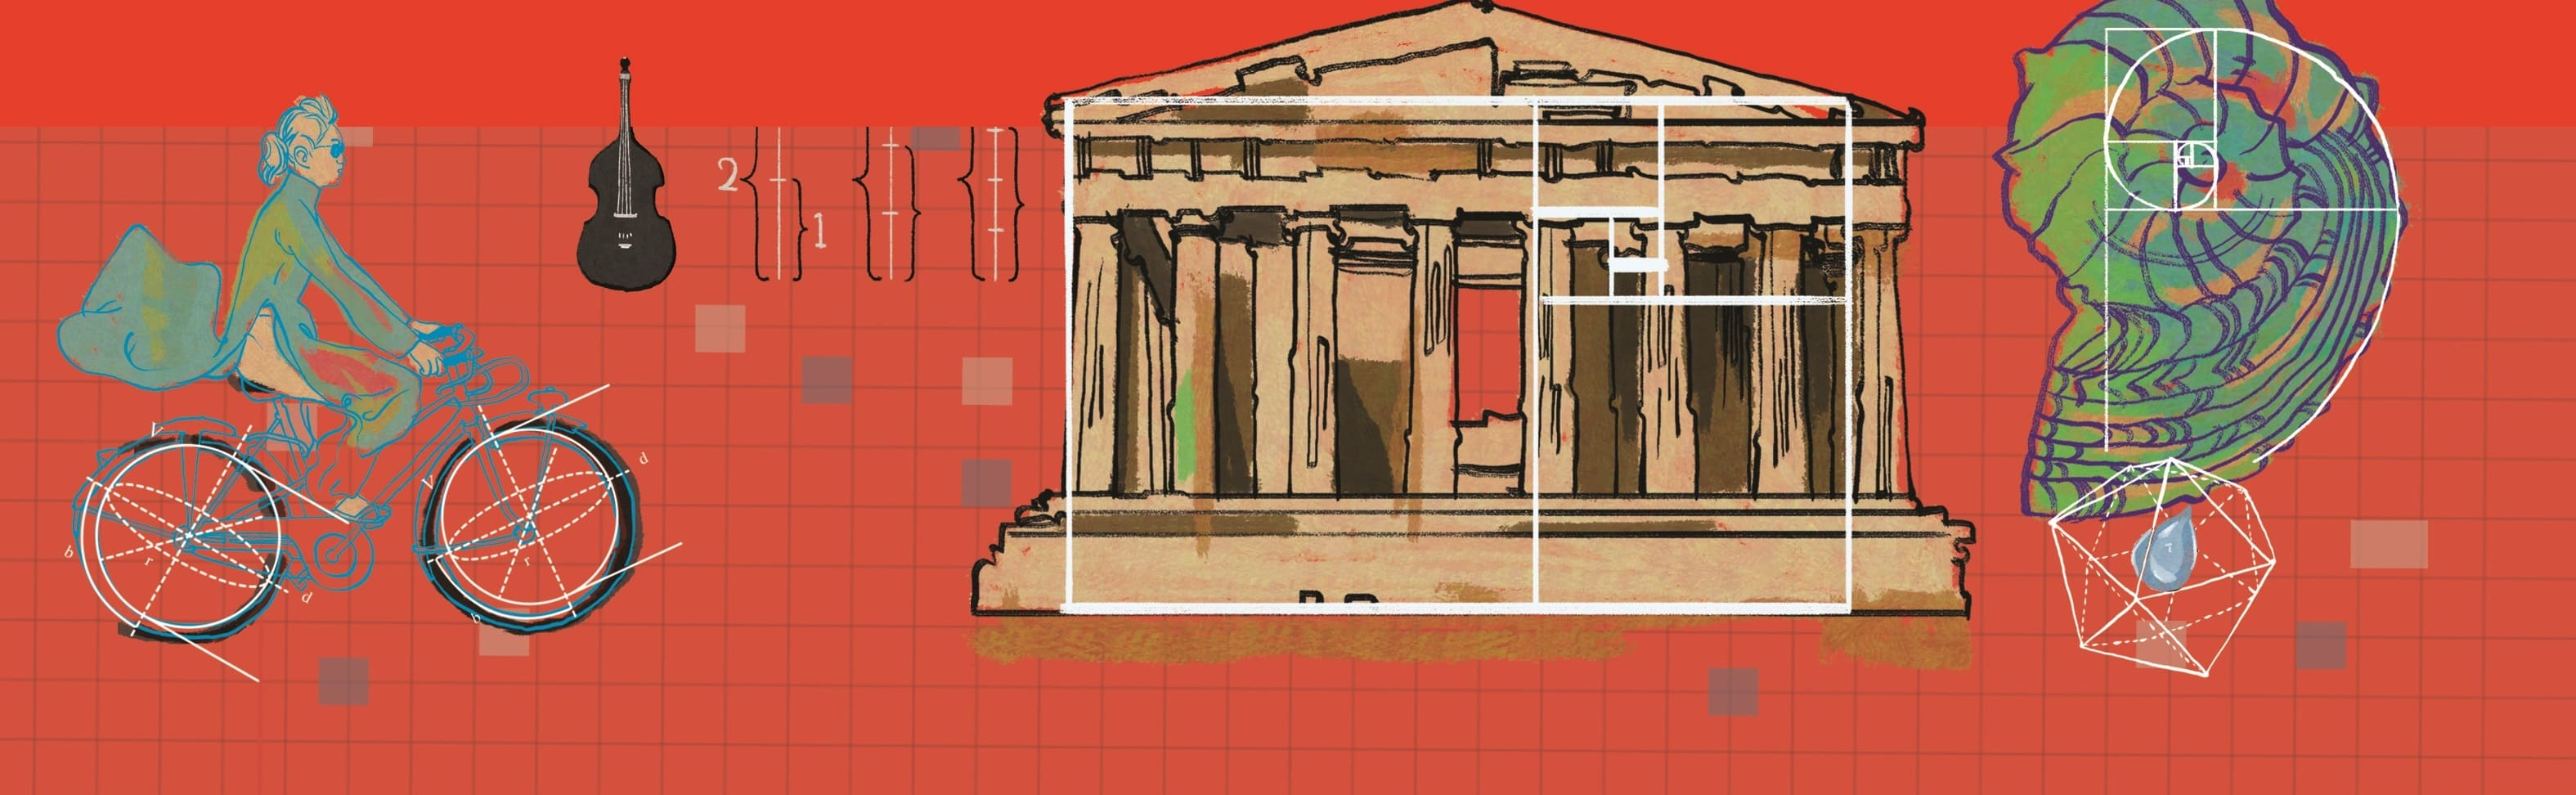
\includegraphics[width=19.3cm]{../bannertoanhocdoisong}}}
\AddToShipoutPicture*{\put(120,525){
\includegraphics[scale=1]{../tieude.pdf}}}
\centering
\endgroup

\vspace*{182pt}

\begin{multicols}{2}
	Việc tính diện tích các miền có dạng đa giác là một hoạt động thường thấy trong đời sống và sản xuất, đặc biệt là với ngành trắc địa. Trong bài viết này, chúng ta hãy cùng tìm hiểu một phương pháp giải bài toán trên dựa vào ``công thức dây giày" cùng một số ứng dụng thú vị khác của công thức này.
	\vskip 0.1cm
	$\pmb{1.}$ \textbf{\color{toanhocdoisong}Trắc địa sử dụng bàn mặt phẳng}
	\vskip 0.1cm
	Trước khi đi sâu vào phương pháp toán học cụ thể để tính diện tích đa giác khi biết tọa độ các đỉnh, chúng ta hãy cùng tìm hiểu cách để thu được vị trí tọa độ các đỉnh của một mảnh đất hình đa giác. Với các công cụ trắc địa hiện đại ngày nay, có nhiều cách thức khác nhau để làm việc này. Tuy nhiên, phần này sẽ trình bày về một công cụ trắc địa có lịch sử tương đối lâu đời: bàn mặt phẳng.
	\vskip 0.1cm
	Bàn mặt phẳng bao gồm một mặt bàn phẳng được đỡ bởi ba chân bàn có thể điều chỉnh được. Kết nối giữa mặt bàn và các chân được thiết kế sao cho mặt bàn có thể quay tự do trong mặt phẳng ngang, đồng thời mặt bàn cũng có thể được điều chỉnh cho song song với mặt đất dựa vào một thiết bị căn chỉnh nào đó, ví dụ một ống bọt nước. Việc chỉnh cho bàn song song với mặt đất là rất quan trọng để đảm bảo tính chính xác của các đo đạc tiếp theo.
	\vskip 0.1cm
	Trên mặt bàn người ta cố định một tờ giấy phẳng. Khi tiến hành đo đạc, mỗi điểm đo đạc trên thực địa sẽ ứng với vị trí tương ứng trên tờ giấy. Để đảm bảo sự tương ứng này khi sử dụng, một kẹp chữ U có buộc dây dọi được gá vào bàn để cho điểm ở trên tờ giấy thẳng hàng đúng với điểm ở trên mặt đất.
	\begin{figure}[H]
		\vspace*{-5pt}
		\centering
		\captionsetup{labelformat= empty, justification=centering}
		
\includegraphics[height= 0.5\linewidth]{1}
		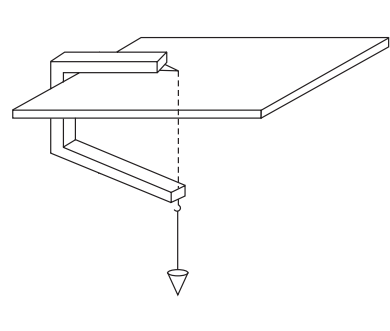
\includegraphics[height= 0.5\linewidth]{2}
		\caption{\small\textit{\color{toanhocdoisong}Hình $1$. Trái: bàn mặt phẳng và các dụng cụ đi kèm. Phải: cách sử dụng công cụ dây dọi đi kèm bàn mặt phẳng.}}
		\vspace*{-10pt}
	\end{figure}
	Tại mỗi một vị trí, người ta sử dụng một thước ngắm để gióng hàng giữa vị trí hiện tại và cọc cắm vị trí được xác định trước đó.
	\vskip 0.1cm
	Khi đã gióng hàng xong, một đường thẳng tương ứng cũng được kẻ trên tờ giấy ở mặt bàn theo đúng phương đã được gióng. Khoảng cách giữa điểm đo mới và điểm đo cũ sẽ bằng đúng khoảng cách thực địa nhân với tỷ lệ xích. Khoảng cách thực địa giữa hai điểm có thể được đo trực tiếp bằng thước dây
	\begin{figure}[H]
		\vspace*{5pt}
		\centering
		\captionsetup{labelformat= empty, justification=centering}
		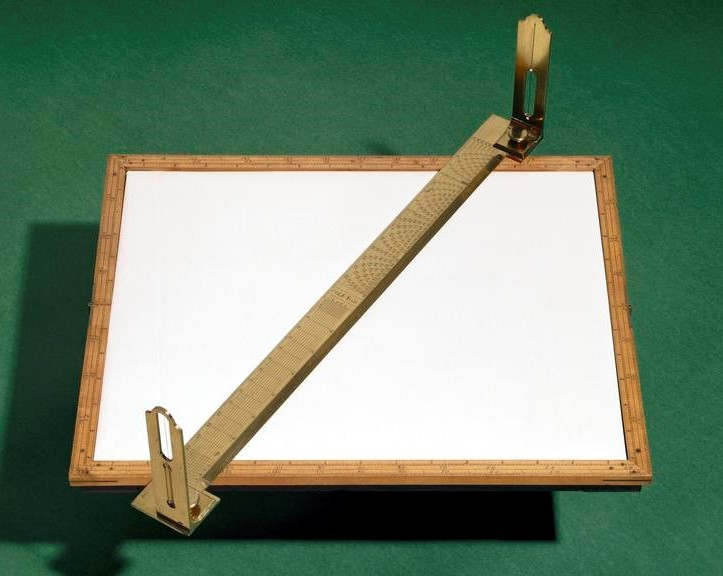
\includegraphics[width= 1\linewidth]{3}
		\caption{\small\textit{\color{toanhocdoisong}Hình $2$. Bàn mặt phẳng với thước ngắm.}}
		\vspace*{-10pt}
	\end{figure}
	hoặc một số phương pháp khác. Một số bàn mặt phẳng sử dụng các ống ngắm có vết đánh dấu còn có thể cho phép xác định khoảng cách bằng các cọc tiêu có chia vạch mà không cần phải nối dây giữa hai điểm. 
	\vskip 0.2cm
	\PIbox{
	\begin{figure}[H]
		\vspace*{-5pt}
		\centering
		\captionsetup{labelformat= empty, justification=centering}
		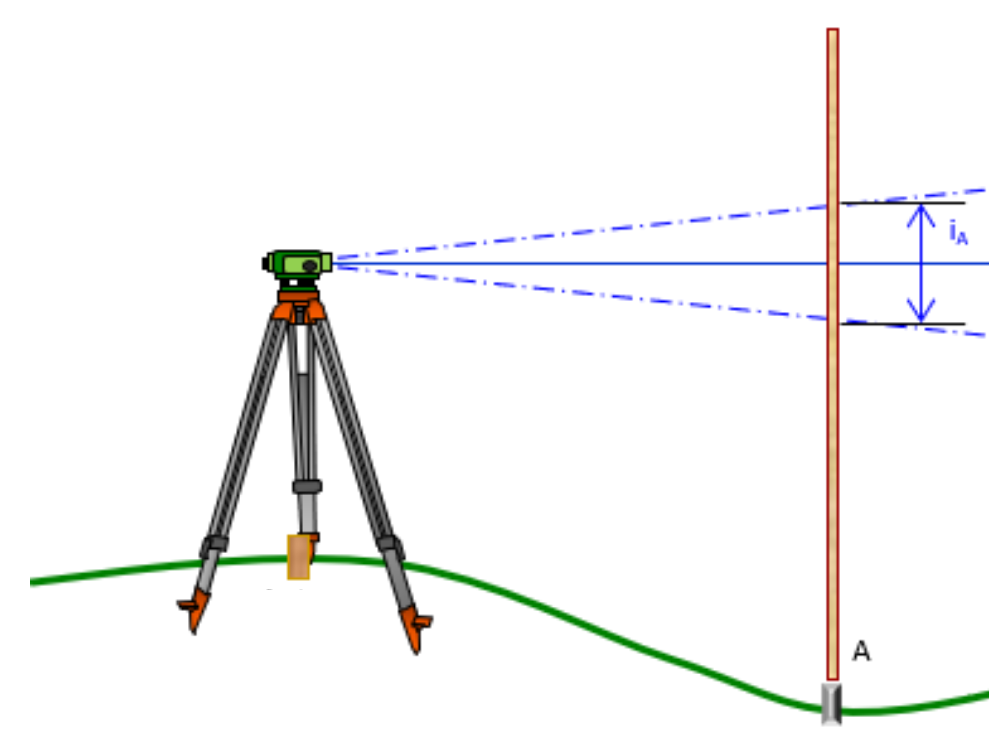
\includegraphics[height= 0.4\linewidth]{4}
		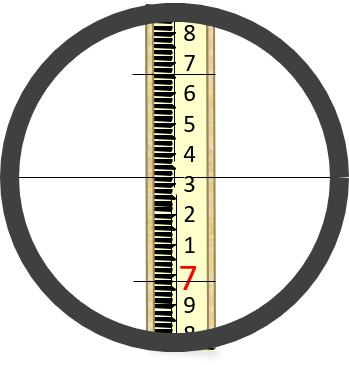
\includegraphics[height= 0.4\linewidth]{5}
%		\caption{\small\textit{\color{}}}
		\vspace*{-10pt}
	\end{figure}
	Khi sử dụng ống ngắm có vạch đánh dấu (còn gọi là vạch \textit{stadia}) để quan sát các cọc tiêu có kẻ vạch, người ta có thể dựa vào khoảng cách quan sát được giữa hai vạch trên cọc để xác định được khoảng cách từ mắt đến cọc thông qua công thức tỷ lệ từ tam giác đồng dạng một cách thuận tiện.
	}
	\vskip 0.2cm
	Nhờ cơ chế trên mà bàn mặt phẳng có thể giúp nhân viên trắc địa lập được một bản đồ sơ bộ theo đúng tỷ lệ xích về vị trí giữa các điểm so với nhau. Việc khảo sát có thể được tiến hành theo nhiều  phương pháp khác nhau:
	\vskip 0.1cm
	$\bullet$ Phương pháp tỏa: người sử dụng bàn mặt phẳng đứng ở một vị trí cố định và xác định vị trí tương đối của các cọc tiêu khác nhau so với vị trí này.
	\begin{figure}[H]
		\vspace*{5pt}
		\centering
		\captionsetup{labelformat= empty, justification=centering}
		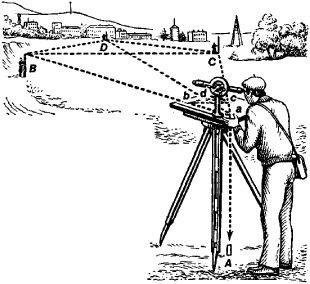
\includegraphics[width= 1\linewidth]{6}
		\caption{\small\textit{\color{toanhocdoisong}Hình $3$. Phương pháp tỏa sử dụng bàn mặt phẳng để xác định tọa độ các vị trí từ một điểm cố định.}}
		\vspace*{-10pt}
	\end{figure}
	$\bullet$ Phương pháp giao điểm: Trong trường hợp có một số điểm không đến được, vị trí của một điểm trên bản đồ được xác định bằng giao của hai đường thẳng từ hai điểm khác đến điểm này. Cách làm này thường sử dụng la bàn để đo độ lệch giữa phương nối hai điểm với hướng Bắc.
	\begin{figure}[H]
		\vspace*{-5pt}
		\centering
		\captionsetup{labelformat= empty, justification=centering}
		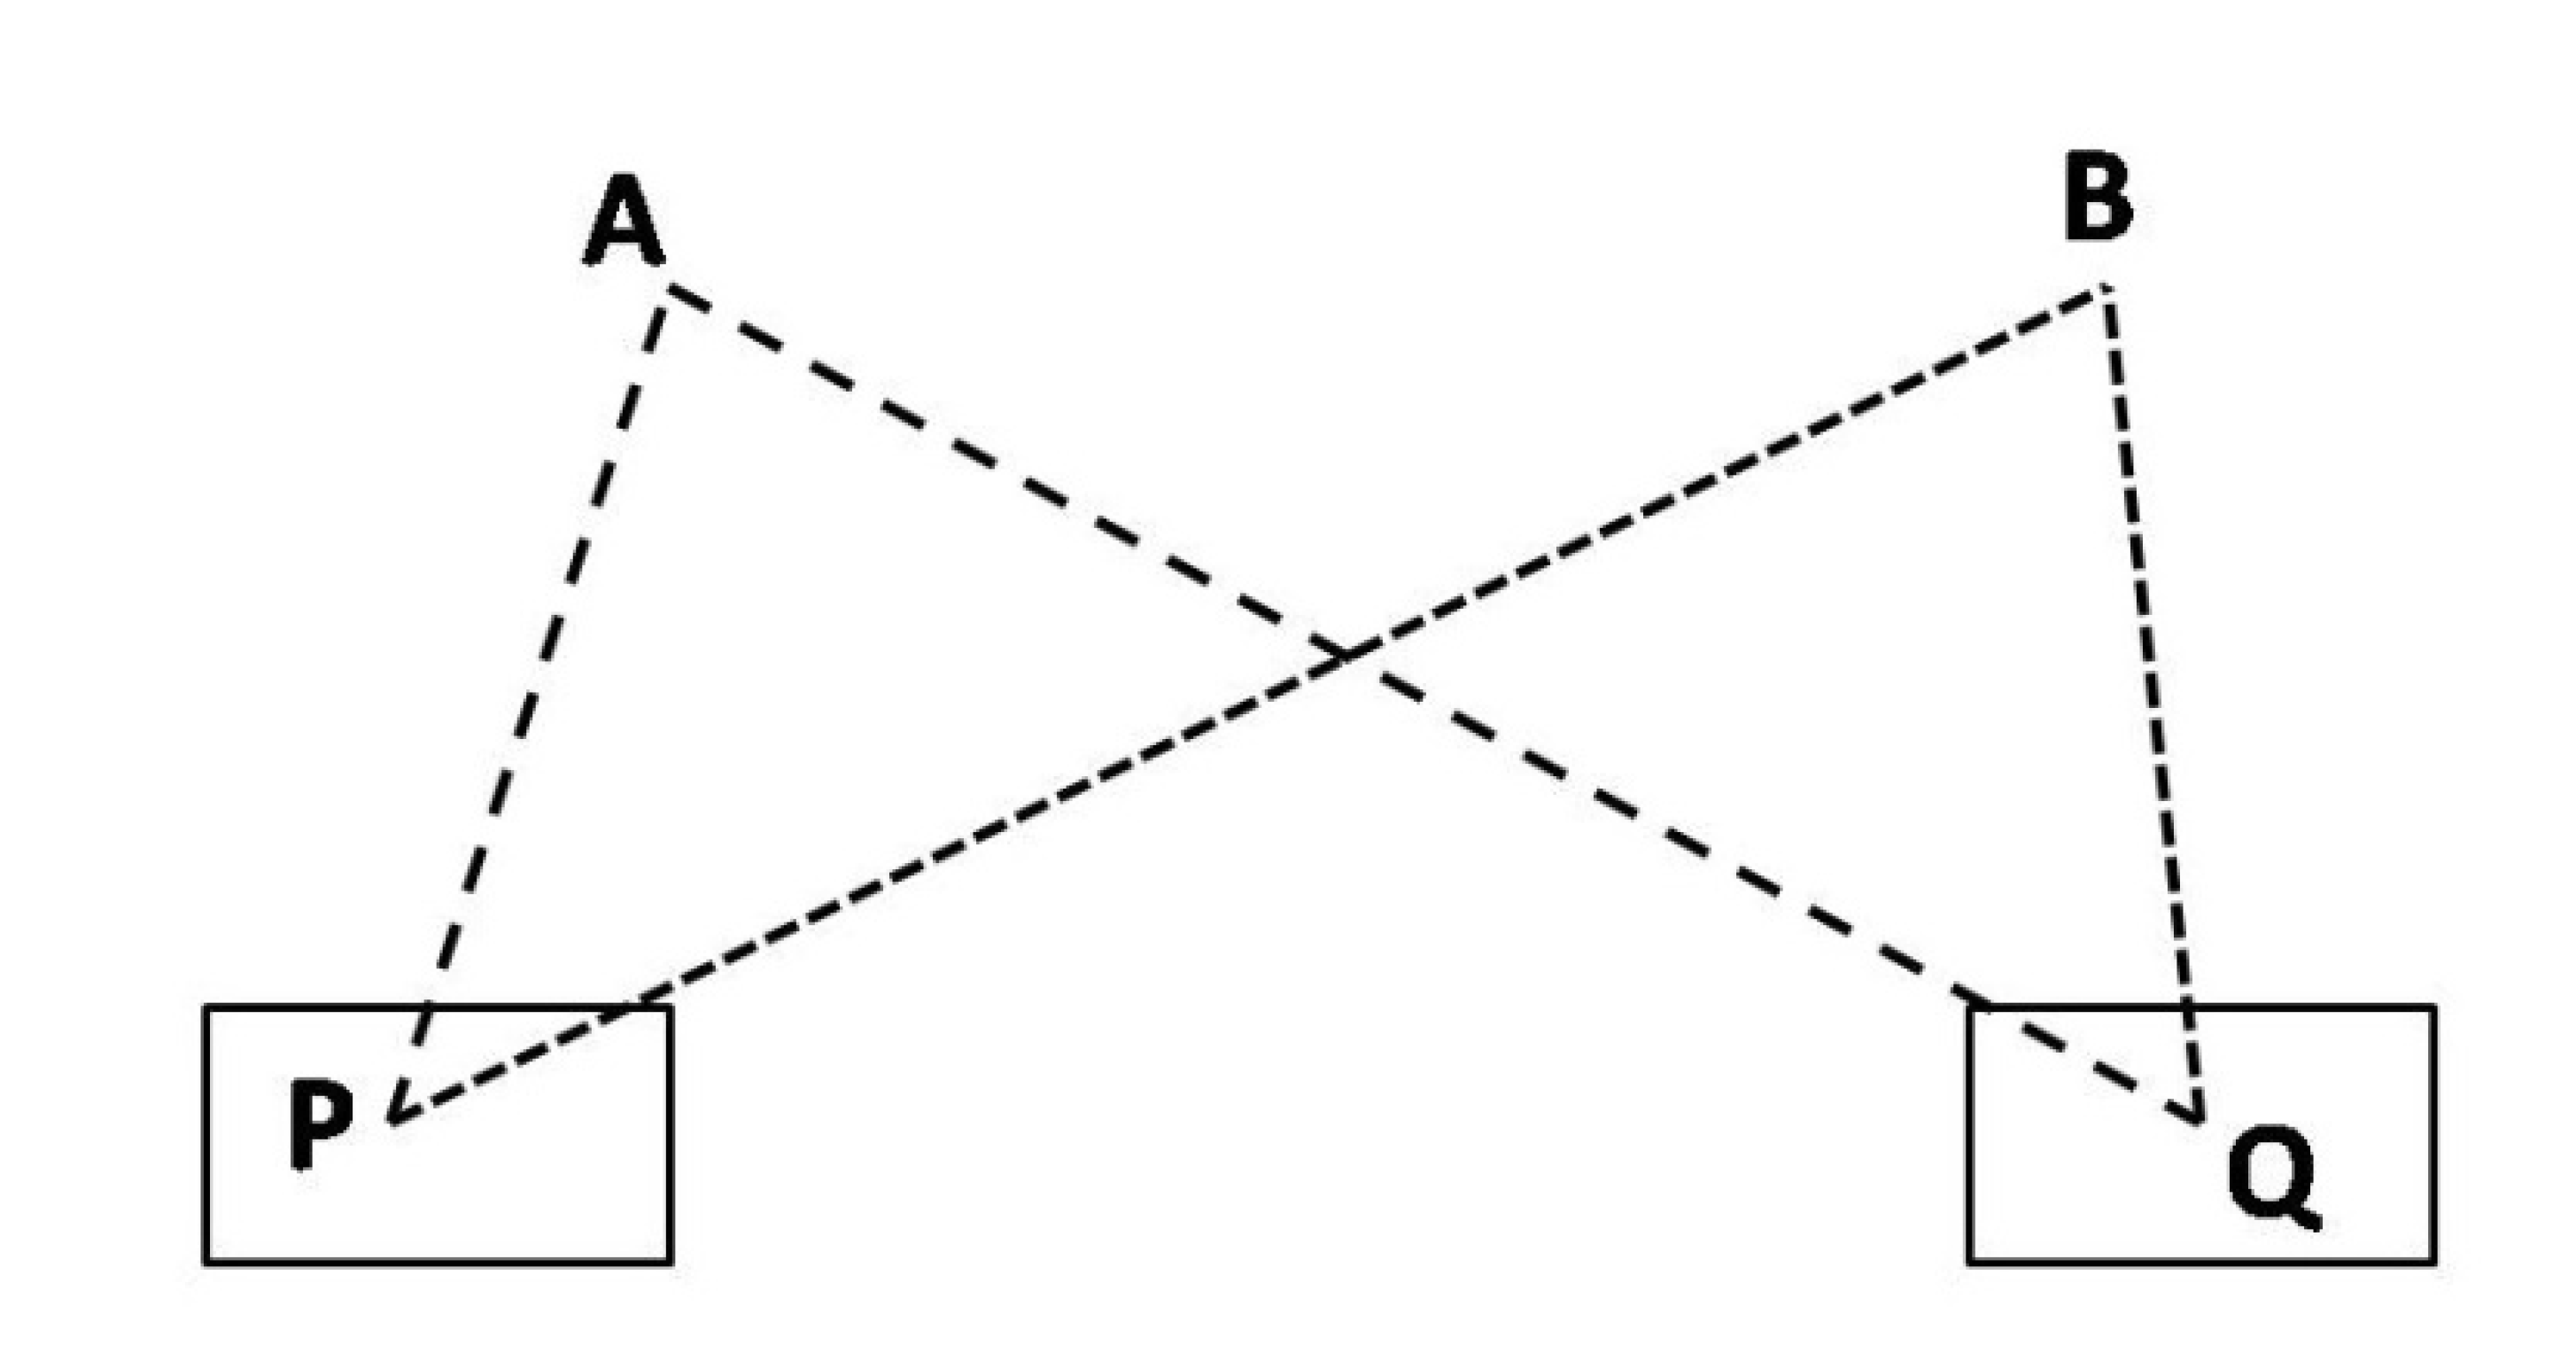
\includegraphics[width= 1\linewidth]{7}
		\caption{\small\textit{\color{toanhocdoisong}Hình $4$. Phương pháp giao điểm sử dụng bàn mặt phẳng từ một số vị trí để xác định tọa độ của các điểm còn lại.}}
		\vspace*{-10pt}
	\end{figure}
	Phương pháp dịch chuyển: Ở mỗi một lần đo, bàn mặt phẳng lại được dịch chuyển đến một vị trí mới. Khi đó, khoảng cách và hướng từ nó đến vị trí cũ lại được đo đạc. Cứ mỗi lần như vậy, ta lại xác định được một cạnh của miền đa giác.
	\begin{figure}[H]
		\vspace*{5pt}
		\centering
		\captionsetup{labelformat= empty, justification=centering}
		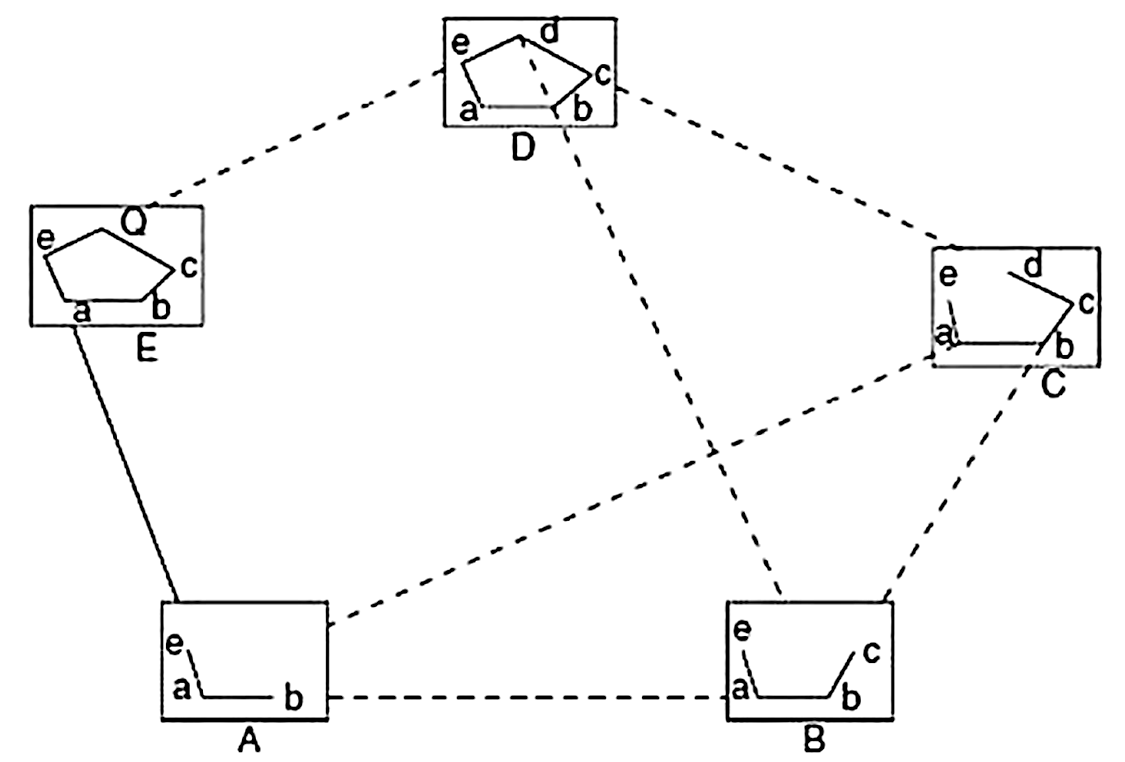
\includegraphics[width= 1\linewidth]{8}
		\caption{\small\textit{\color{toanhocdoisong}Hình $5$. Phương pháp dịch chuyển xác định tọa độ các điểm bằng cách dịch chuyển bàn mặt phẳng và gióng lại điểm ngay trước. Các điểm trước hơn nữa cũng có thể được sử dụng để hiệu chỉnh khoảng cách.}}
		\vspace*{-10pt}
	\end{figure}
	\vskip 0.1cm
	\begin{tBox}
		\begin{wrapfigure}{l}{0.4\linewidth}
			\vspace*{-15pt}
			\centering
			\captionsetup{labelformat= empty, justification=centering}
			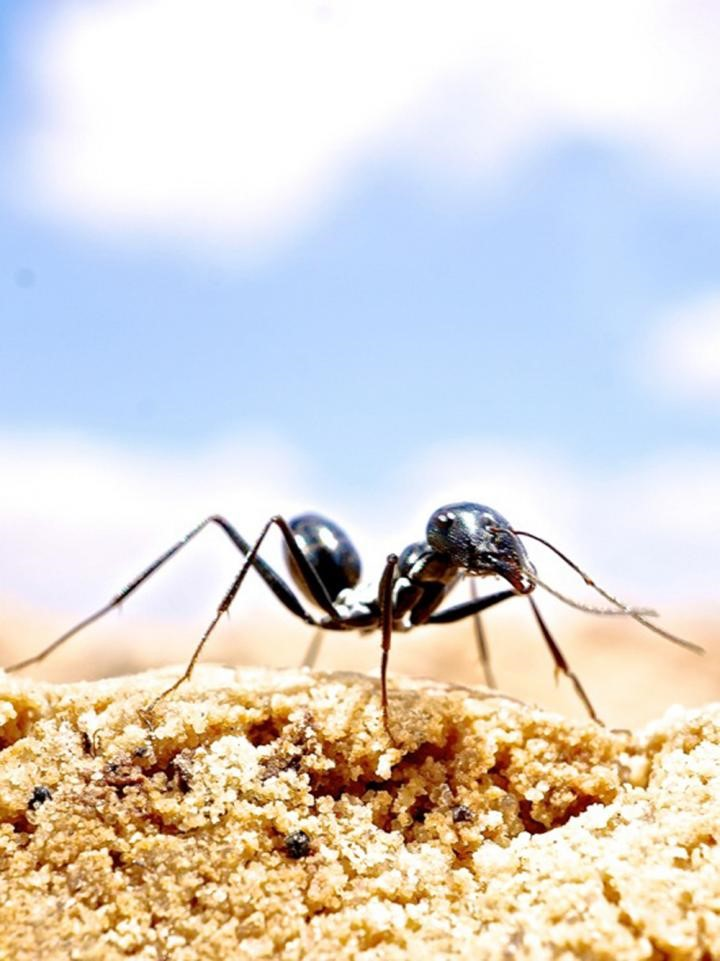
\includegraphics[width= 1\linewidth]{9}
			%		\caption{\small\textit{\color{}}}
			\vspace*{-20pt}
		\end{wrapfigure}	
		Một số nghiên cứu sinh học cho thấy loài kiến sa mạc (Cataglyphis fortis) cũng định vị bằng một cách tương tự như trên, chúng có thể xác định được hướng và khoảng cách giữa một số mốc cố định để không bị lạc đường trong sa mạc.
	\end{tBox}
	\vskip 0.1cm
	Bàn mặt phẳng xuất hiện từ giai đoạn cuối thể kỷ $16$, đầu thế kỷ $17$. Tuy rằng đã có nhiều công cụ tiên tiến hơn nhưng đặc tính đơn giản, thuận tiện, dễ sử dụng vẫn giúp bàn mặt phẳng được sử dụng trong nhiều trường hợp khác nhau khi tiến hành trắc địa.
	\vskip 0.1cm
	$\pmb{2.}$ \textbf{\color{toanhocdoisong}Công thức dây giày: tính diện tích đa giác từ tọa độ các đỉnh}
	\vskip 0.1cm
	Như đã thấy ở phần trên, bằng một phương pháp trắc địa nào đó, ví dụ như bàn mặt phẳng, ta có thể thu được một bản đồ dạng tỷ lệ xích của miền đa giác, cũng như tọa độ các đỉnh của nó. Để tính diện tích miền đa giác này, một suy nghĩ thông thường là hãy chia nó thành các tam giác rồi tính diện tích từng tam giác này. Dù sao thì độ dài của mỗi cạnh có thể thu được bằng định lý Pythagoras và diện tích mỗi tam giác có thể được tính từ độ dài ba cạnh qua công thức Heron.
	\vskip 0.1cm
	Tuy nhiên, còn có cách tính diện tích nào với khối lượng tính toán ít hơn không? Nếu đã biết tọa độ của tất cả các đỉnh trong một hệ trục tọa độ Descartes, ta có thể tính diện tích đa giác theo công thức sau:
	\begin{align*}
		S \!=\! \dfrac{1}{2}\!\left(\begin{vmatrix}
			x_1 \!&\!\! x_2\\
			y_1 \!&\!\! y_2
		\end{vmatrix} \!+\! \cdots \!+\! \begin{vmatrix}
		x_{n-1} \!&\!\! x_n\\
		y_{n-1} \!&\!\! y_n
	\end{vmatrix} + \begin{vmatrix}
	x_n \!&\!\! x_1\\
	y_n \!&\!\! y_1
	\end{vmatrix}\right)
	\end{align*}
	với ($x_i,y_i$) là tọa độ của đỉnh $A_i$ của đa giác $A_1 A_2 A_3\ldots A_n$.
	\vskip 0.05cm
	Ở đây, các định thức $2\times2$ có giá trị được tính theo công thức sau:
	\begin{align*}
		\begin{matrix}
			a & b\\
			c & d
		\end{matrix} = ad - bc.
	\end{align*}
	\begin{figure}[H]
		\vspace*{-5pt}
		\centering
		\captionsetup{labelformat= empty, justification=centering}
		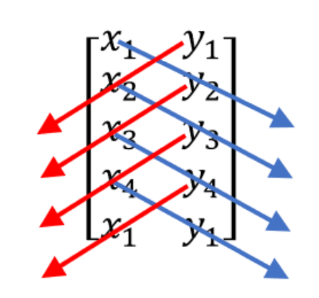
\includegraphics[width= 1\linewidth]{10}
		\caption{\small\textit{\color{toanhocdoisong}Hình 6. Minh họa công thức dây giày.}}
		\vspace*{-10pt}
	\end{figure}
	Đây còn gọi là công thức dây giày vì cách thức nhân chéo giống với cách buộc dây giày (Hình $6$). Nó còn được gọi là công thức tính diện tích của Gauss. Công thức này có nhiều cách chứng minh khác nhau. Ở đây, ta hãy cùng tìm hiểu một cách chứng minh tương đối đơn giản sử dụng các kiến thức toán sơ cấp.
	\vskip 0.05cm
	Xét hai vector $u$ và $v$ như trong Hình $7$. Góc $\theta$ khi quay từ $u$ đến $v$ sẽ dương khi chiều quay ngược kim đồng hồ và âm khi chiều quay cùng chiều kim đồng hồ. Ta có thể tính sinθ theo công thức lượng giác:
	\begin{align*}
		\sin\theta =& \sin(\theta_2 - \theta1)\\
		= &\sin\theta_2\cos\theta_1 - \sin\theta_1\cos\theta_2\\
		= &\frac{d}{||v||}\cdot\frac{a}{||u||} - \frac{b}{||u||}\cdot\frac{c}{||v||}\\
		= &\dfrac{1}{||u||\cdot ||v||}(ad - bc).
	\end{align*}
	Ở đây $||u||$ và $||v||$ lần lượt là độ dài của các vector tương ứng.
	\vskip 0.1cm
	Ta đã biết diện tích của một hình bình hành bằng với tích của độ dài hai cạnh nhân với $\sin$ của góc giữa chúng. Để phục vụ các tính toán tiếp theo, ta sẽ dùng khái niệm diện tích có dấu:
	\begin{align*}
		||u||||v||\sin\theta = ad - bc.
	\end{align*}
	Diện tích này sẽ dương nếu chiều quay từ u đến v là ngược chiều kim đồng hồ và âm nếu chiều quay ngược lại.
	\begin{figure}[H]
		\vspace*{-5pt}
		\centering
		\captionsetup{labelformat= empty, justification=centering}
		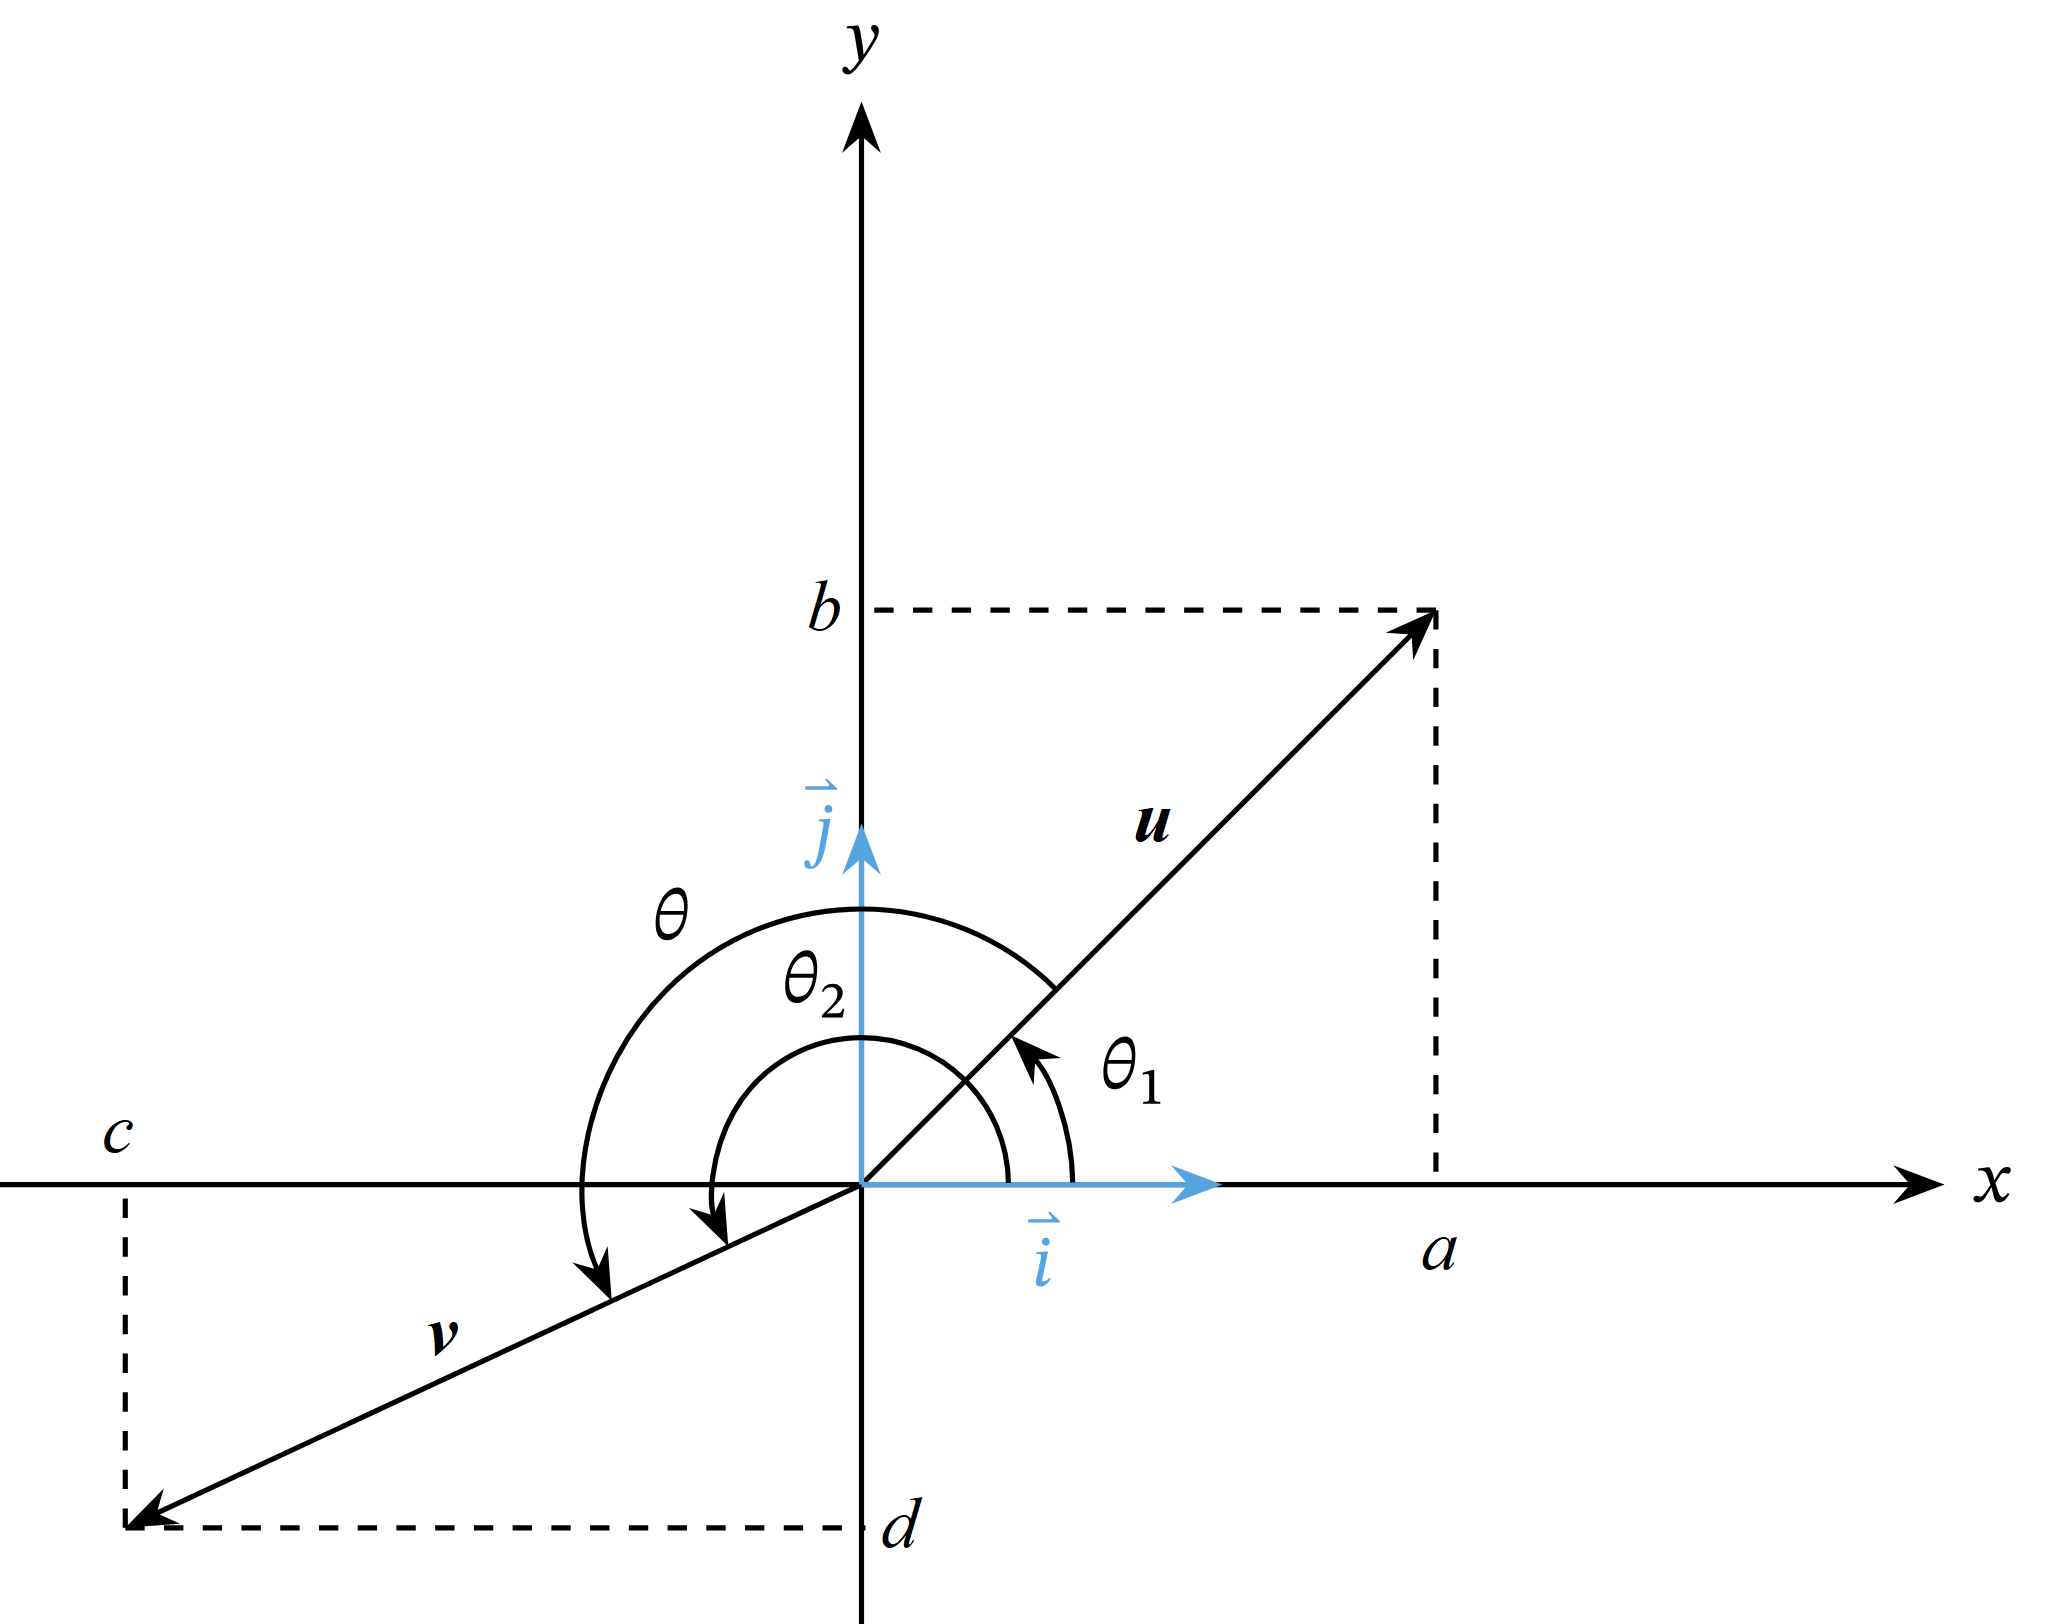
\includegraphics[width= 1\linewidth]{11}
		\caption{\small\textit{\color{toanhocdoisong}Hình $7$. Góc giữa mỗi vector với trục $x$ và góc giữa hai vector.}}
		\vspace*{-10pt}
	\end{figure}
	Do diện tích tam giác bằng một nửa diện tích hình bình hành có chung hai cạnh, diện tích có dấu của tam giác tạo bởi hai vector $u$ và $v$ là:
	\begin{align*}
		\dfrac{1}{2}(ad-bc).
	\end{align*}
	Trong trường hợp tam giác tạo bởi hai vector $(x_1,y_1)$ và $(x_2,y_2)$, ta có diện tích tam giác (có dấu) tính theo công thức:
	\begin{align*}
		\dfrac{1}{2}(x_1y_2 - x_2y_1).
	\end{align*}
	Diện tích này dương khi chiều quay từ vector $(x_1,y_1)$ đến $(x_2,y_2)$ là ngược chiều kim đồng hồ và âm trong trường hợp ngược lại.
	\vskip 0.1cm
	Từ công thức này, ta hãy mở rộng cho trường hợp một đa giác lồi có chứa gốc tọa độ ở miền trong của nó. Giả sử tọa độ các đỉnh của đa giác là $A_1(x_1,y_1),A_2 (x_2,y_2),\ldots,A_n(x_n,y_n)$ theo thứ tự ngược chiều kim đồng hồ.
	\vskip 0.1cm
	Khi đó diện tích có dấu của đa giác sẽ bằng tổng diện tích có dấu của các tam giác:
	\begin{align*}
		&\dfrac{1}{2}(x_1y_2 - x_2y_1 + x_2y_3 - x_3y_2 + \cdots \\
		&+ x_{n-1}y_n - x_ny_{n-1} + x_ny_1 - x_1y_n).
	\end{align*}
	và sẽ nhận giá trị dương.
	\begin{figure}[H]
		\vspace*{-5pt}
		\centering
		\captionsetup{labelformat= empty, justification=centering}
		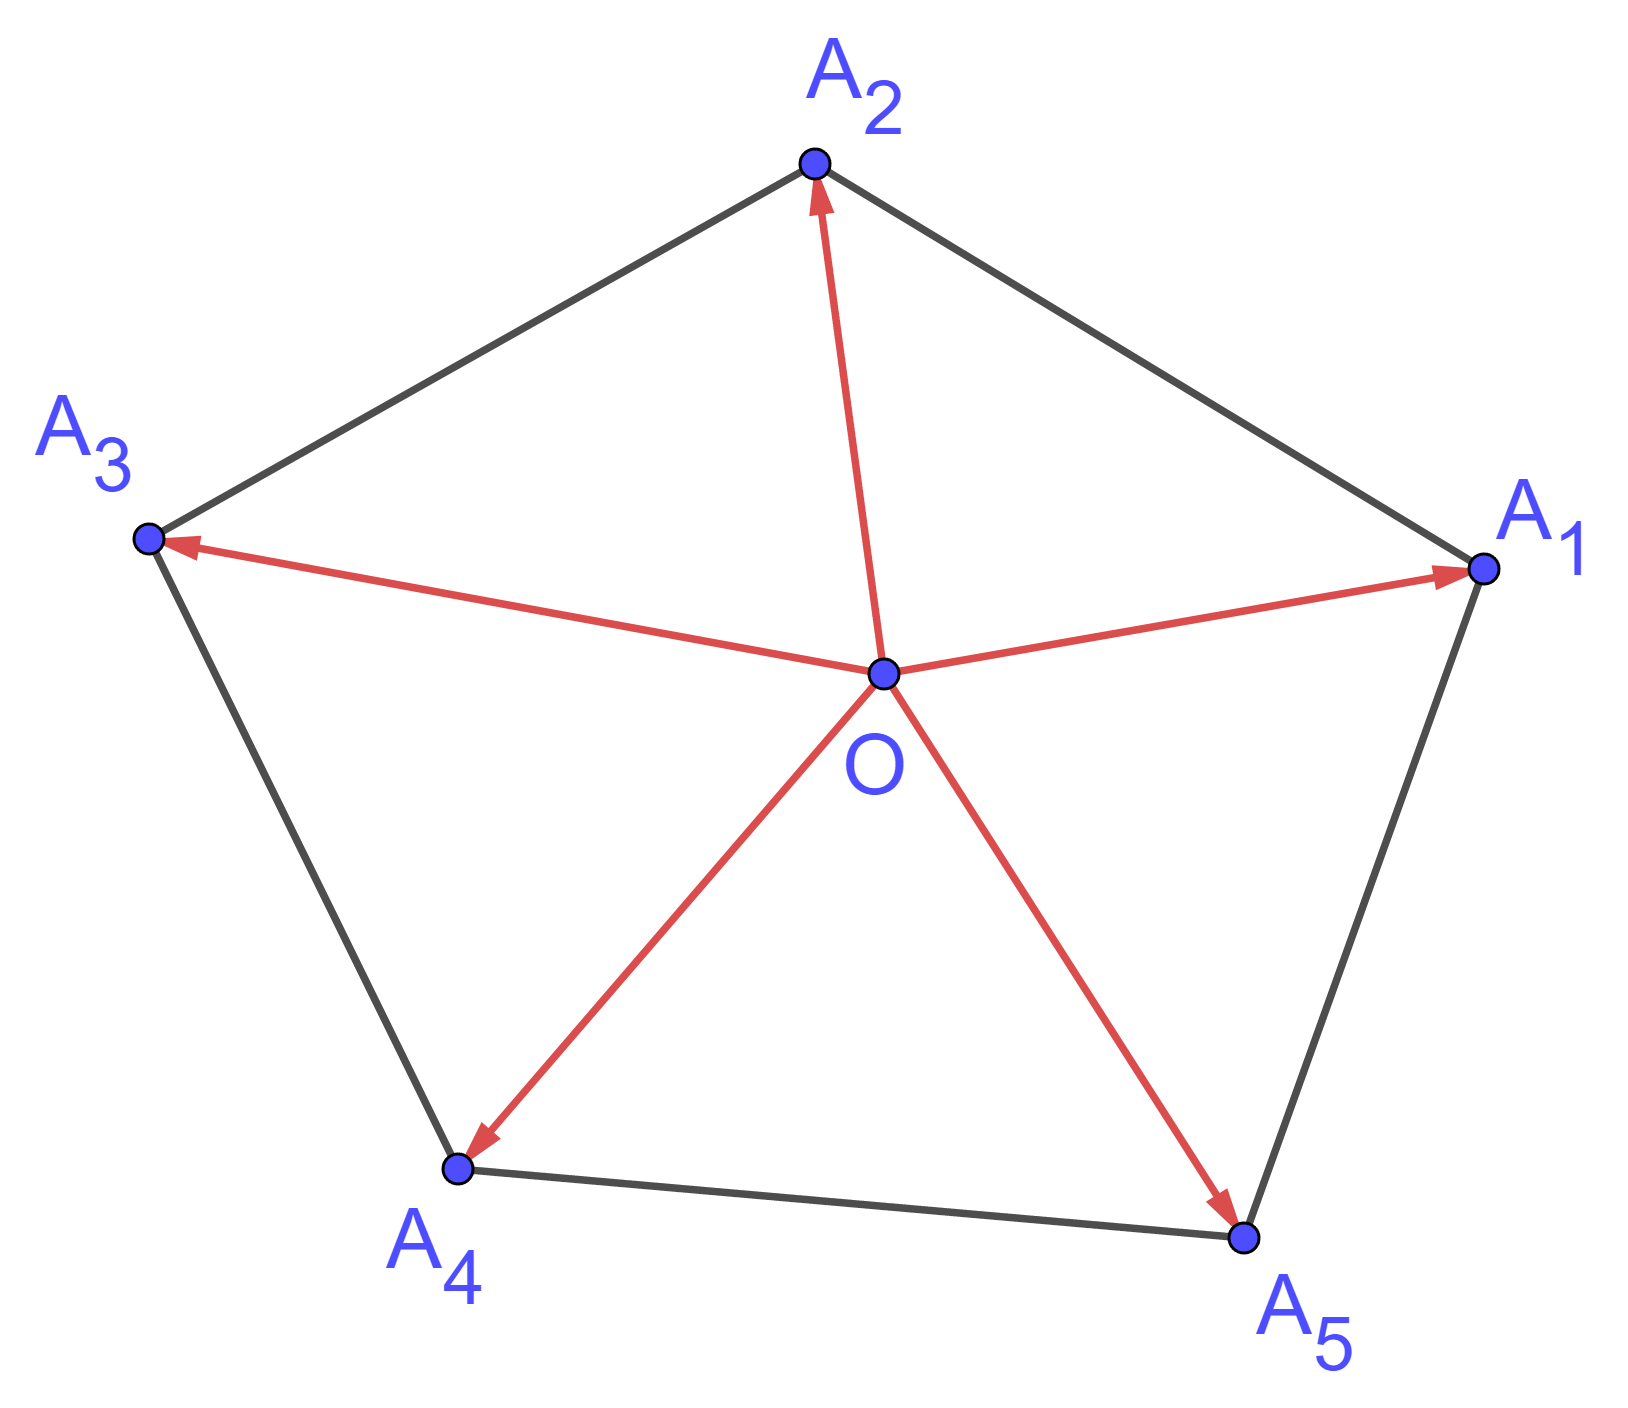
\includegraphics[width= 1\linewidth]{12}
		\caption{\small\textit{\color{toanhocdoisong}Hình $8$. Trường hợp đa giác lồi có gốc tọa độ ở miền trong đa giác.}}
		\vspace*{-10pt}
	\end{figure}
	Tất nhiên không phải đa giác nào cũng chứa gốc tọa độ ở miền trong của nó. Với trường hợp này, ta hãy để ý rằng với $u=(a,b),v=(c,d)$ thì $ad-bc$ cũng chính là thành phần theo trục $z$ của tích có hướng $u\cdot v$. Giả sử $O$ không còn là gốc tọa độ mà chỉ là một điểm bất kỳ ở miền trong tam giác, các vector từ $O$ đến các đỉnh đa giác lần lượt là $v_1,v_2,\ldots,v_n$ còn vector từ gốc tọa độ đến $O$ là $w$.
	\vskip 0.1cm
	Ta có:
	\begin{align*}
		&(v_1+w) \times (v_2+w)+(v_2+w) \times (v_3+w)\\
		&+ \cdots +(v_n+w) \times (v_1+w)\\
		&(v_1 \times v_2+v_2 \times v_3+\cdots+v_{n-1} \times v_n + v_n \times v_1 )\\
		&+(v_1+v_2+\cdots+v_{n-1}+v_n) \times w \\
		&+ w \times (v_1+v_2+\cdots +v_{n-1}+v_n)\\
		&(v_1 \times v_2+v_2 \times v_3+\cdots + v_{n-1} \times v_n + v_n \times v_1)
	\end{align*}
	Ở đây ta đã sử dụng tính chất $a \times b=-b \times a$ để triệt tiêu các thành phần có tích vô hướng liên quan đến $w$.
	\vskip 0.1cm
	Biểu thức trên cũng chỉ ra rằng dù gốc tọa độ không nằm trong đa giác thì công thức dây giày vẫn cho cho ta diện tích của đa giác.
	\begin{figure}[H]
		\vspace*{-5pt}
		\centering
		\captionsetup{labelformat= empty, justification=centering}
		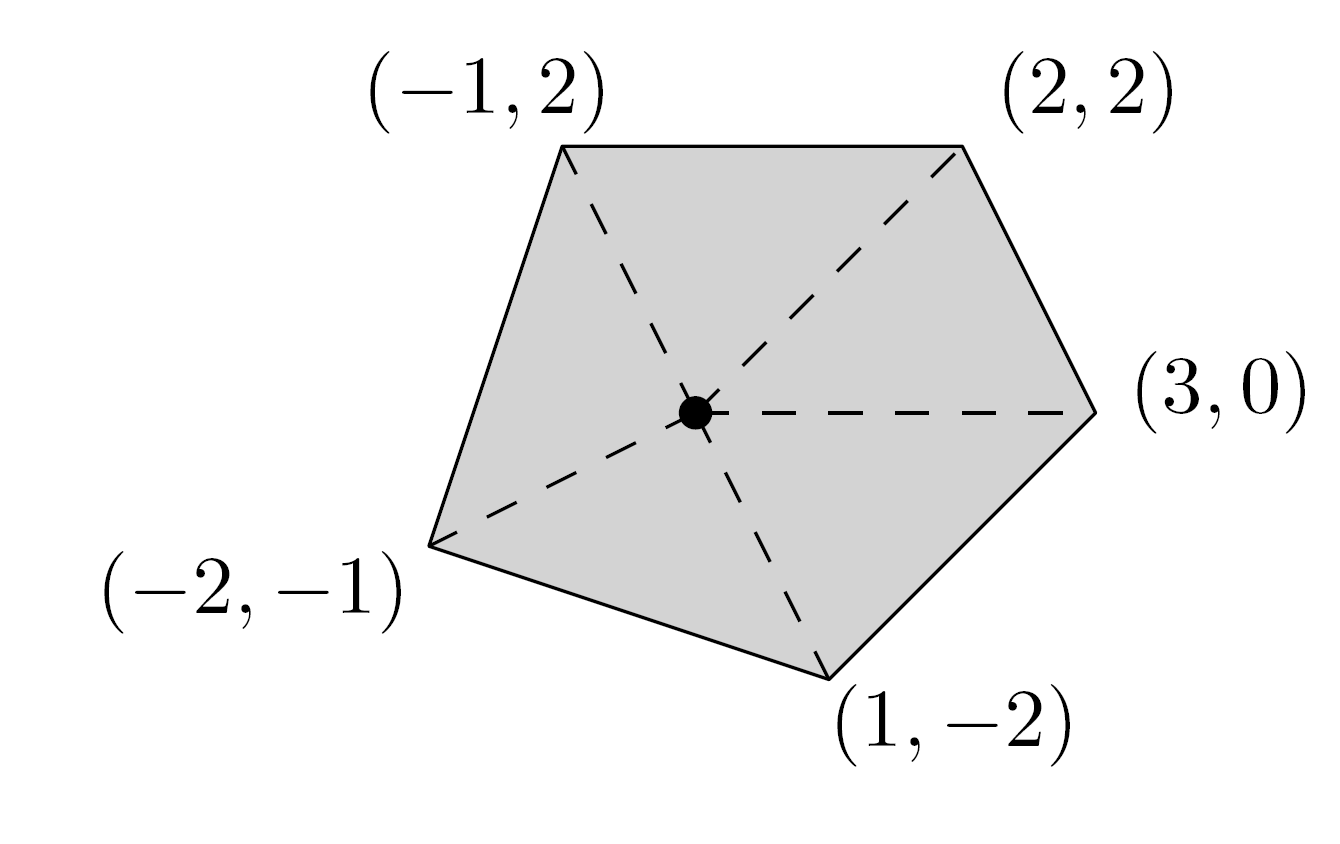
\includegraphics[width= 1\linewidth]{13}
		\caption{\small\textit{\color{toanhocdoisong}Hình $9$. Một ví dụ tính diện tích sử dụng công thức dây giày.}}
		\vspace*{-10pt}
	\end{figure}
	Ví dụ với đa giác có tọa độ các đỉnh như trong Hình $9$, sau khi thay số vào công thức, ta được giá trị diện tích là $14$ (nếu các đỉnh được liệt kê theo thứ tự ngược chiều kim đồng hồ).
	\vskip 0.1cm
	Trong trường hợp đa giác là không lồi, công thức dây giày vẫn đúng. Các tam giác có thứ tự liệt kê các đỉnh cùng chiều kim đồng hồ sẽ có diện tích âm. Các phần âm dương sẽ bù trừ cho nhau và công thức dây giày vẫn cho ta diện tích của đa giác.
	\begin{figure}[H]
		\vspace*{-5pt}
		\centering
		\captionsetup{labelformat= empty, justification=centering}
		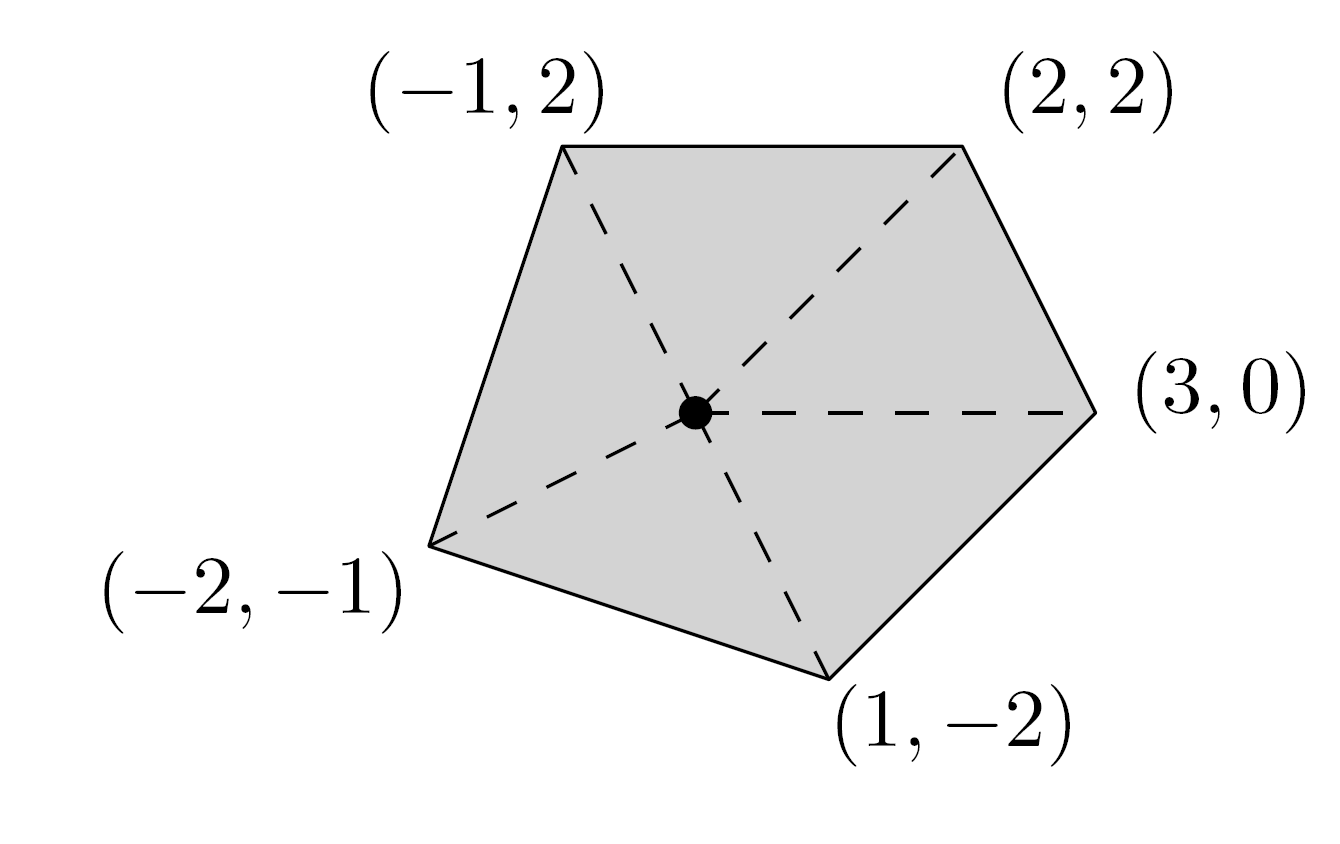
\includegraphics[width= 1\linewidth]{13}
		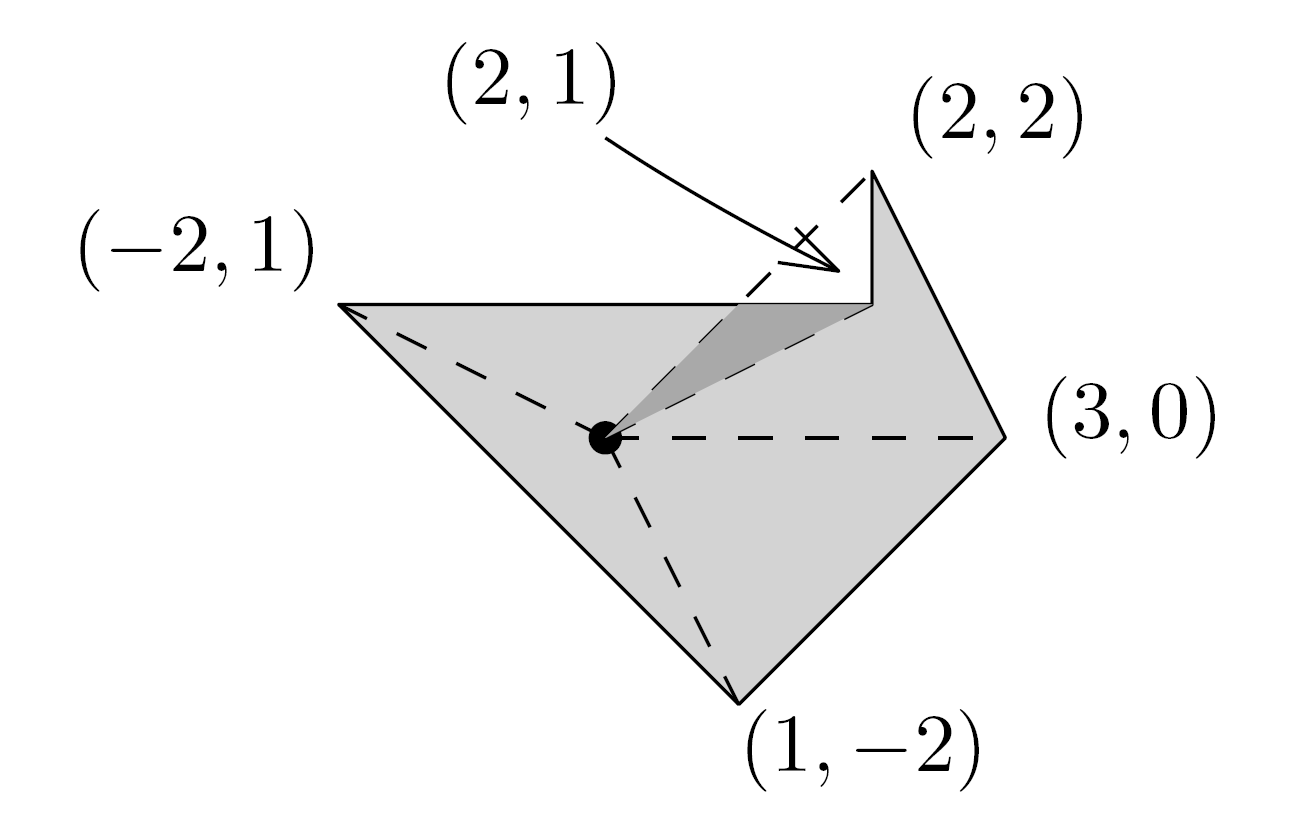
\includegraphics[width= 1\linewidth]{14}
		\caption{\small\textit{\color{toanhocdoisong}Hình $10$. Minh họa công thức dây giày cho trường hợp đa giác không lồi.}}
		\vspace*{-10pt}
	\end{figure}
	Do đặc điểm bù trừ này mà công thức dây giày cũng vẫn đúng cho trường hợp đa giác có các cạnh cắt nhau như trong Hình $11$.
	\begin{figure}[H]
		\vspace*{-5pt}
		\centering
		\captionsetup{labelformat= empty, justification=centering}
		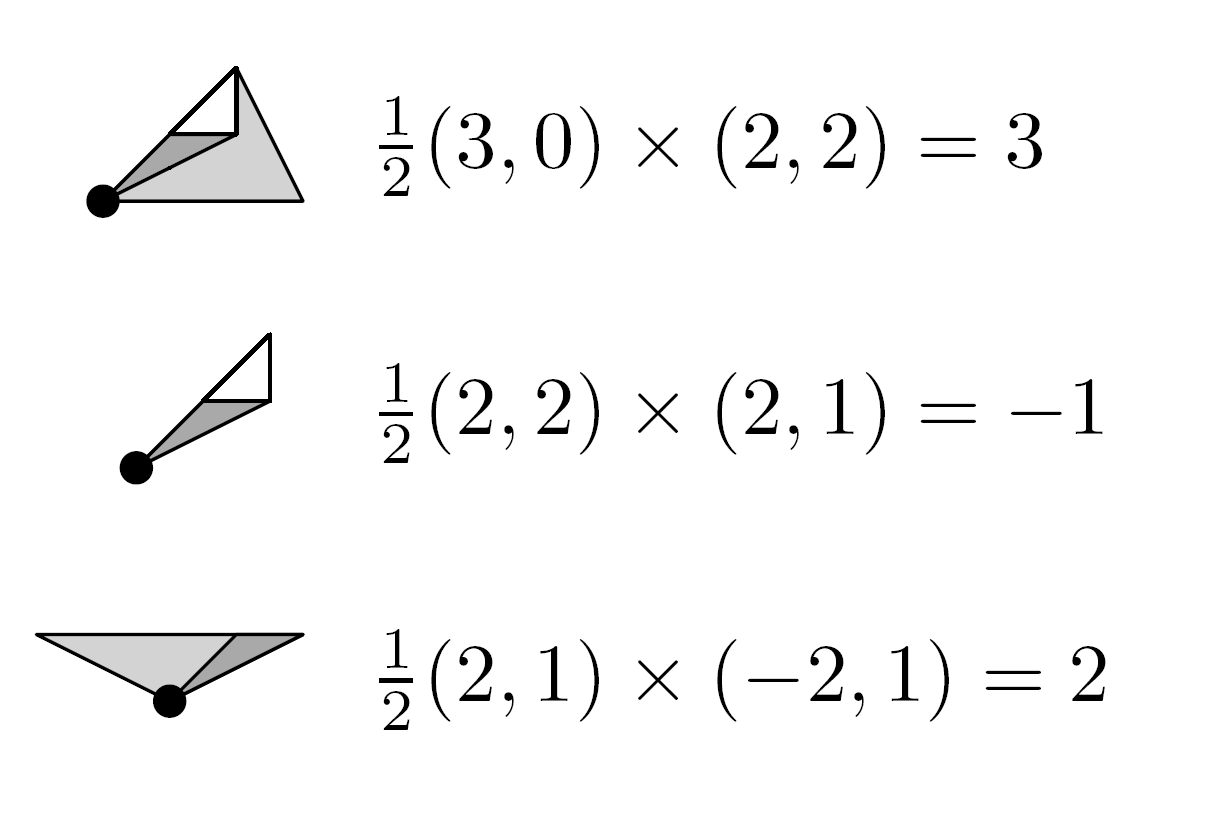
\includegraphics[width= 1\linewidth]{15}
		\caption{\small\textit{\color{toanhocdoisong}Hình $11$. Công thức dây giày vẫn đúng trong trường hợp đa giác có các cạnh cắt nhau.}}
		\vspace*{-10pt}
	\end{figure}
	Ta cũng có thể tiến hành chứng minh công thức dây giày theo một cách tiếp cận khác. Xét hai đỉnh $(x_i,y_i)$ và $(x_(i+1),y_(i+1))$ của một đa giác có các đỉnh nằm hoàn toàn phía trên trục $x$. Đây là hai đỉnh liền nhau. Biểu thức  $\dfrac{1}{2}(x_{i+1}-x_i)(y_i+y_{i+1})$ chính là một diện tích có dấu của hình thang bao gồm cạnh nối hai đỉnh này, hai đoạn vuông góc hạ từ các đỉnh xuống trục $x$, và hình chiếu của cạnh này trên trục $x$ (Hình $12$). Ngược lại với chứng minh trên, diện tích này sẽ dương khi chiều từ $(x_i,y_i)$ sang $(x_{i+1},y_{i+1})$ là cùng chiều kim đồng hồ (hướng từ trái sang phải trên cạnh của đa giác) và âm trong trường hợp ngược lại. Tất nhiên nó sẽ bằng $0$ khi cạnh đa giác vuông góc với trục $x$.
	\begin{figure}[H]
		\vspace*{-5pt}
		\centering
		\captionsetup{labelformat= empty, justification=centering}
		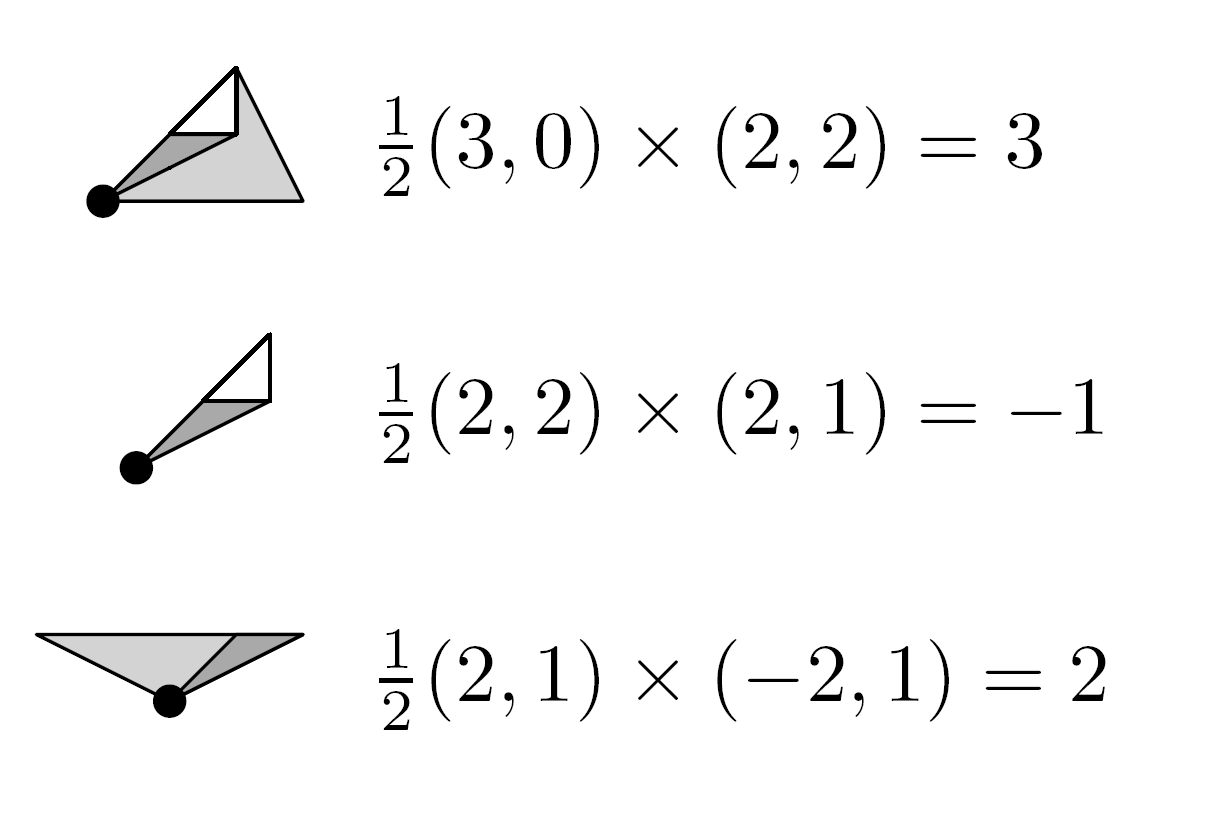
\includegraphics[width= 1\linewidth]{15}
		\caption{\small\textit{\color{toanhocdoisong}Hình $12$. Chứng minh công thức dây giày dựa vào diện tích hình thang.}}
		\vspace*{-10pt}
	\end{figure}
	Khi tiến hành cộng tổng diện tích tất cả các hình thang được sinh ra theo cách này và rút gọn lại biểu thức, ta cũng sẽ thu được công thức tính diện tích theo tọa độ. Thật vậy:
	\begin{align*}
		&\frac{1}{2}\sum\limits_{i = 1}^n \left( {{x_{i + 1}} - {x_i}} \right)\left( {{y_{i + 1}} + {y_i}} \right) \\
		= &\frac{1}{2}\sum\limits_{i = 1}^n \left( {{x_{i + i}}{y_{i + 1}} + {x_{i + 1}}{y_i} - {x_i}{y_{i + 1}} + {x_i}{y_i}} \right) \\
		= &\frac{1}{2}\left( {\sum\limits_{i = 1}^n {{x_{i + i}}{y_i} - } \sum\limits_{i = 1}^n {{x_i}{y_{i + 1}}} } \right) .
	\end{align*}
	Chú ý rằng công thức này ngược dấu so với công thức dây giày ban đầu do các đỉnh được liệt kê theo chiều kim đồng hồ thay vì ngược chiều kim đồng hồ.
	\vskip 0.1cm
	Trong trường hợp đa giác không hoàn toàn nằm phía trên trục $x$, ta cần chứng minh rằng công thức này cho giá trị không đổi khi dịch gốc tọa độ dọc theo trục thẳng đứng. Giả sử tất cả các tọa độ trên trục y của mỗi điểm đều được cộng thêm một lượng là $C$. Khi đó:
	\begin{align*}
		&\frac{1}{2}\sum\limits_{i = 1}^n \left( {{x_{i + 1}} - {x_i}} \right)\left( {{y_{i + 1}} + {y_i} + 2C} \right) \\
		= &\frac{1}{2}\sum\limits_{i = 1}^n \left( {{x_{i + 1}} - {x_i}} \right)\left( {{y_{i + 1}} + {y_i}} \right) + 2C\left( {{x_{i + 1}} - {x_i}} \right) \\
		= &\frac{1}{2} \sum\limits_{i = 1}^n \left( {{x_{i + 1}} - {x_i}} \right)\left( {{y_{i + 1}} + {y_i}} \right) + C \cdot \sum\limits_{i = 1}^n {\left( {{x_{i + 1}} - {x_i}} \right)}  \\
	= &\frac{1}{2}\sum\limits_{i = 1}^n {\left( {{x_{i + 1}} - {x_i}} \right)\left( {{y_{i + 1}} + {y_i}} \right)} 
	\end{align*}
	Số hạng chứa $C$ bằng $0$ do $x_{n+1}$ cũng chính là $x_1$ (các cạnh đa giác tạo thành một đường gấp khúc khép kín). Phương pháp chứng minh sử dụng hình thang này cũng đúng cho trường hợp đa giác không lồi (Hình $13$).
	\begin{figure}[H]
		\vspace*{-10pt}
		\centering
		\captionsetup{labelformat= empty, justification=centering}
		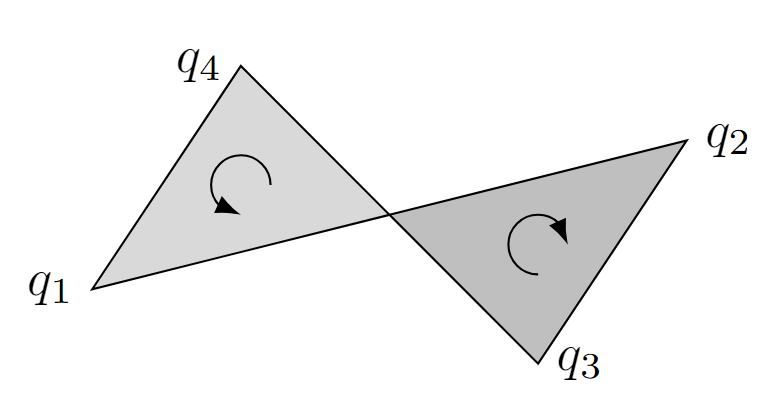
\includegraphics[width= 0.9\linewidth]{16}
		\caption{\small\textit{\color{toanhocdoisong}Hình $13$. Các hình thang trong trường hợp đa giác không lồi.}}
		\vspace*{-10pt}
	\end{figure}
	Một ứng dụng đáng chú ý của công thức dây giày là nó cho ta định lý Pythagoras một cách trực tiếp. 
	\begin{figure}[H]
		\vspace*{-5pt}
		\centering
		\captionsetup{labelformat= empty, justification=centering}
		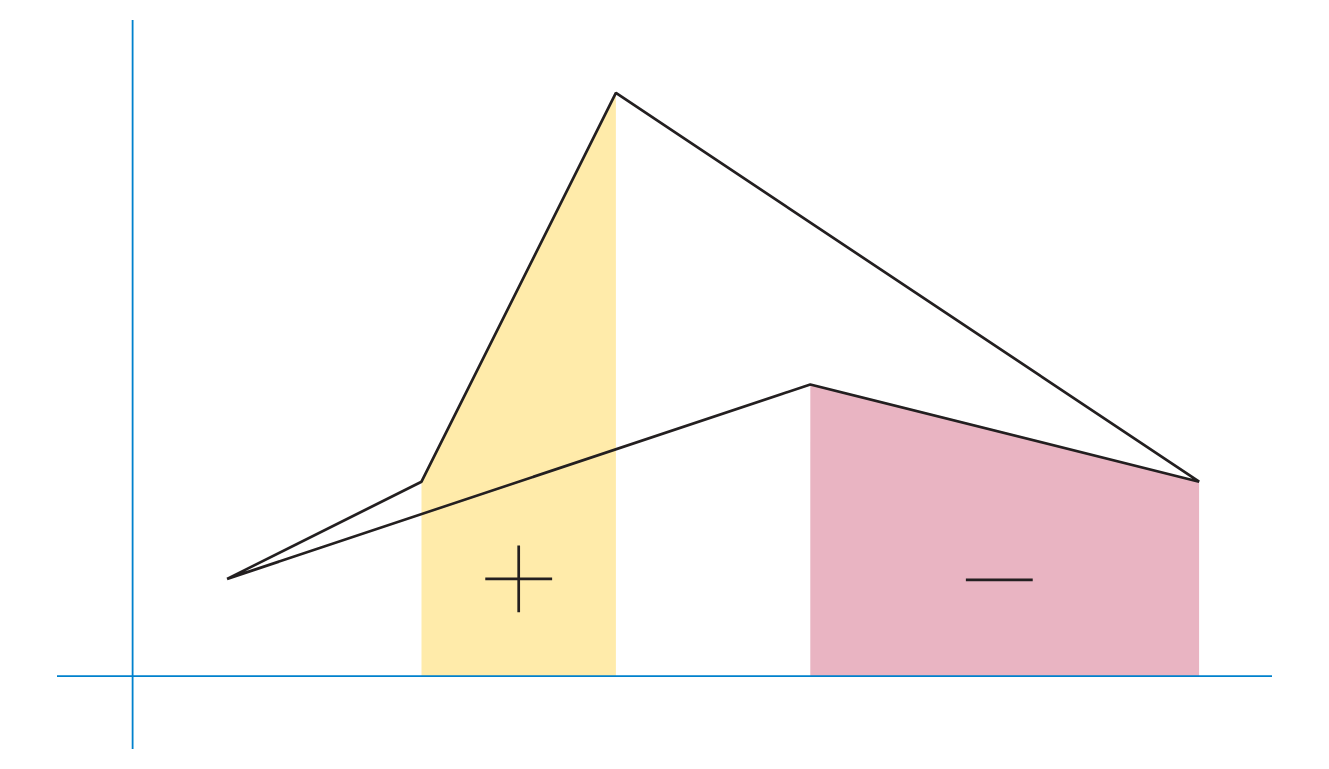
\includegraphics[width= 0.9\linewidth]{17}
		\caption{\small\textit{\color{toanhocdoisong}Hình $14$. Sử dụng công thức dây giày để chứng minh định lý Pythagoras.}}
		\vspace*{-10pt}
	\end{figure}
	Xét tam giác vuông $OAB$ với tọa độ các đỉnh $O(0,0)$, $A(a,0)$, $B(0,b)$. Có thể dễ dàng chứng minh bằng hình học rằng các đỉnh của hình vuông $ABCD$ trong hình có tọa độ là $C(b,a+b)$ và $D(a+b,a)$.
	\vskip 0.1cm
	Diện tích hình vuông $ABCD$ có thể được tính theo công thức dây giày theo thứ tự liệt kê $A, D, C, B$:
	\begin{align*}
		&\dfrac{1}{2}\left[a\cdot a - 0 \cdot(a+b) + (a+b)\cdot(a+b) \right.\\
		&\left.- a\cdot b + b\cdot b - (a+b)\cdot 0 + 0 \cdot 0 - a\cdot b\right]\\
		=\,\, &a^2 + b^2.
	\end{align*}
	Đồng thời diện tích hình vuông này cũng bằng $c^2$ với $c=AB$, và định lý Pythagoras đã được chứng minh.
	\vskip 0.1cm
	\textbf{\color{toanhocdoisong}Bài tập}
	\vskip 0.1cm
	$\pmb{1.}$ Dùng công thức dây giày, tính diện tích của các đa giác với các đỉnh có tọa độ như sau:
	\vskip 0.05cm
	$a)$ $(1,1)$, $(2,4)$, $(0,6)$.
	\vskip 0.1cm
	$b)$ $(1,3)$, $(-1,2)$, $(-3, -6)$, $(0,-1)$.
	\vskip 0.1cm
	$c)$ $(2,2)$, $(-2,2)$, $(-4, -4)$, $(0,-2)$, $(4,-4)$.
	\vskip 0.1cm
	$\pmb{2.}Ư$ Liên hệ giữa định thức và diện tích hình bình hành cũng có thể được chứng minh bằng cách cắt ghép trực quan. Hình bên dưới mô tả cách làm này cho trường hợp $0<b<d$, $0<c<a$. Bạn đọc hãy liệt kê các trường hợp còn lại và tiến hành chứng minh dùng cắt ghép cho các trường hợp này.
	\begin{figure}[H]
		\vspace*{-5pt}
		\centering
		\captionsetup{labelformat= empty, justification=centering}
		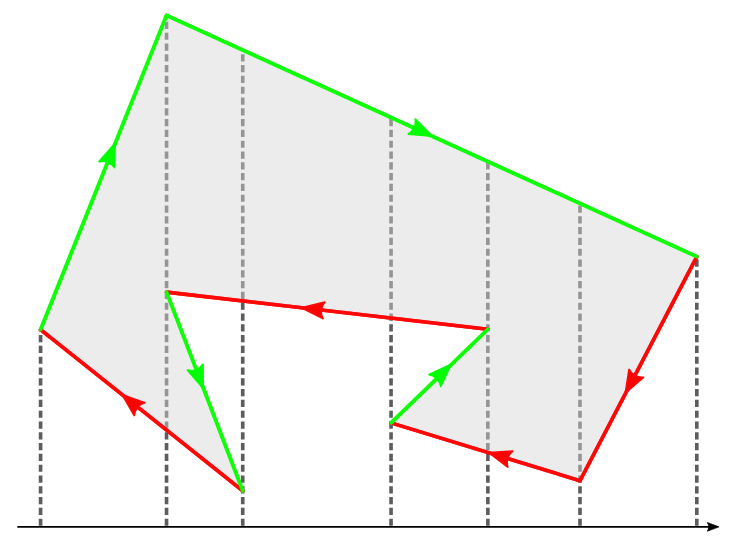
\includegraphics[width= 0.8\linewidth]{18}
		\vspace*{-10pt}
	\end{figure}
	$\pmb{3.}$ \textbf{\color{toanhocdoisong}Diện tích của miền bao bởi đường cong kín}
	\vskip 0.1cm
	Sau khi đã giải quyết bài toán tính diện tích của một đa giác, ta hãy giải quyết bài toán tính diện tích của miền được bao bởi một đường cong kín. Trước hết, ta hãy bàn về cách mô tả một đường cong kín như thế nào. Do đường cong kín chắc chắn không thể mô tả bằng một hàm số dạng $y=f(x)$ (vì trong trường hợp này ứng với một giá trị của $x$ có thể có nhiều hơn một giá trị của $y$) nên ta cần một cách khác để mô tả đường cong.
	\vskip 0.1cm
	Nhiều đường cong quen thuộc có thể được mô tả bằng dạng tham số (giống như dạng tham số của đường thẳng trong sách giáo khoa toán). Theo đó, một đường cong có thể được biểu diễn dưới dạng $(x(t),y(t))$ với $t\in [a,b]$ là tham số mô tả đường cong.
	\vskip 0.1cm
	Ví dụ, đường tròn bán kính $R$ có tâm ở gốc tọa độ sẽ có dạng tham số $(R\cos t,R\sin t), t\in [0,2\pi]$. Còn đường ellipse có dạng tham số $(a\cos t,b\sin t), t\in [0,2\pi]$ với $a,b$ lần lượt là độ dài các bán trục ngang và đứng.
	\vskip 0.1cm
	Xét một đường cong kín $(x(t),y(t))$ với $t \in [a,b]$ và khi $t$ tăng thì vị trí điểm tương ứng với giá trị  này sẽ đi dọc đường cong theo chiều dương (ngược chiều kim đồng hồ). Xét các điểm $t_i$:
	\begin{align*}
		a=t_0<t_1<\ldots<t_n=b
	\end{align*}
	\begin{figure}[H]
		\vspace*{-5pt}
		\centering
		\captionsetup{labelformat= empty, justification=centering}
		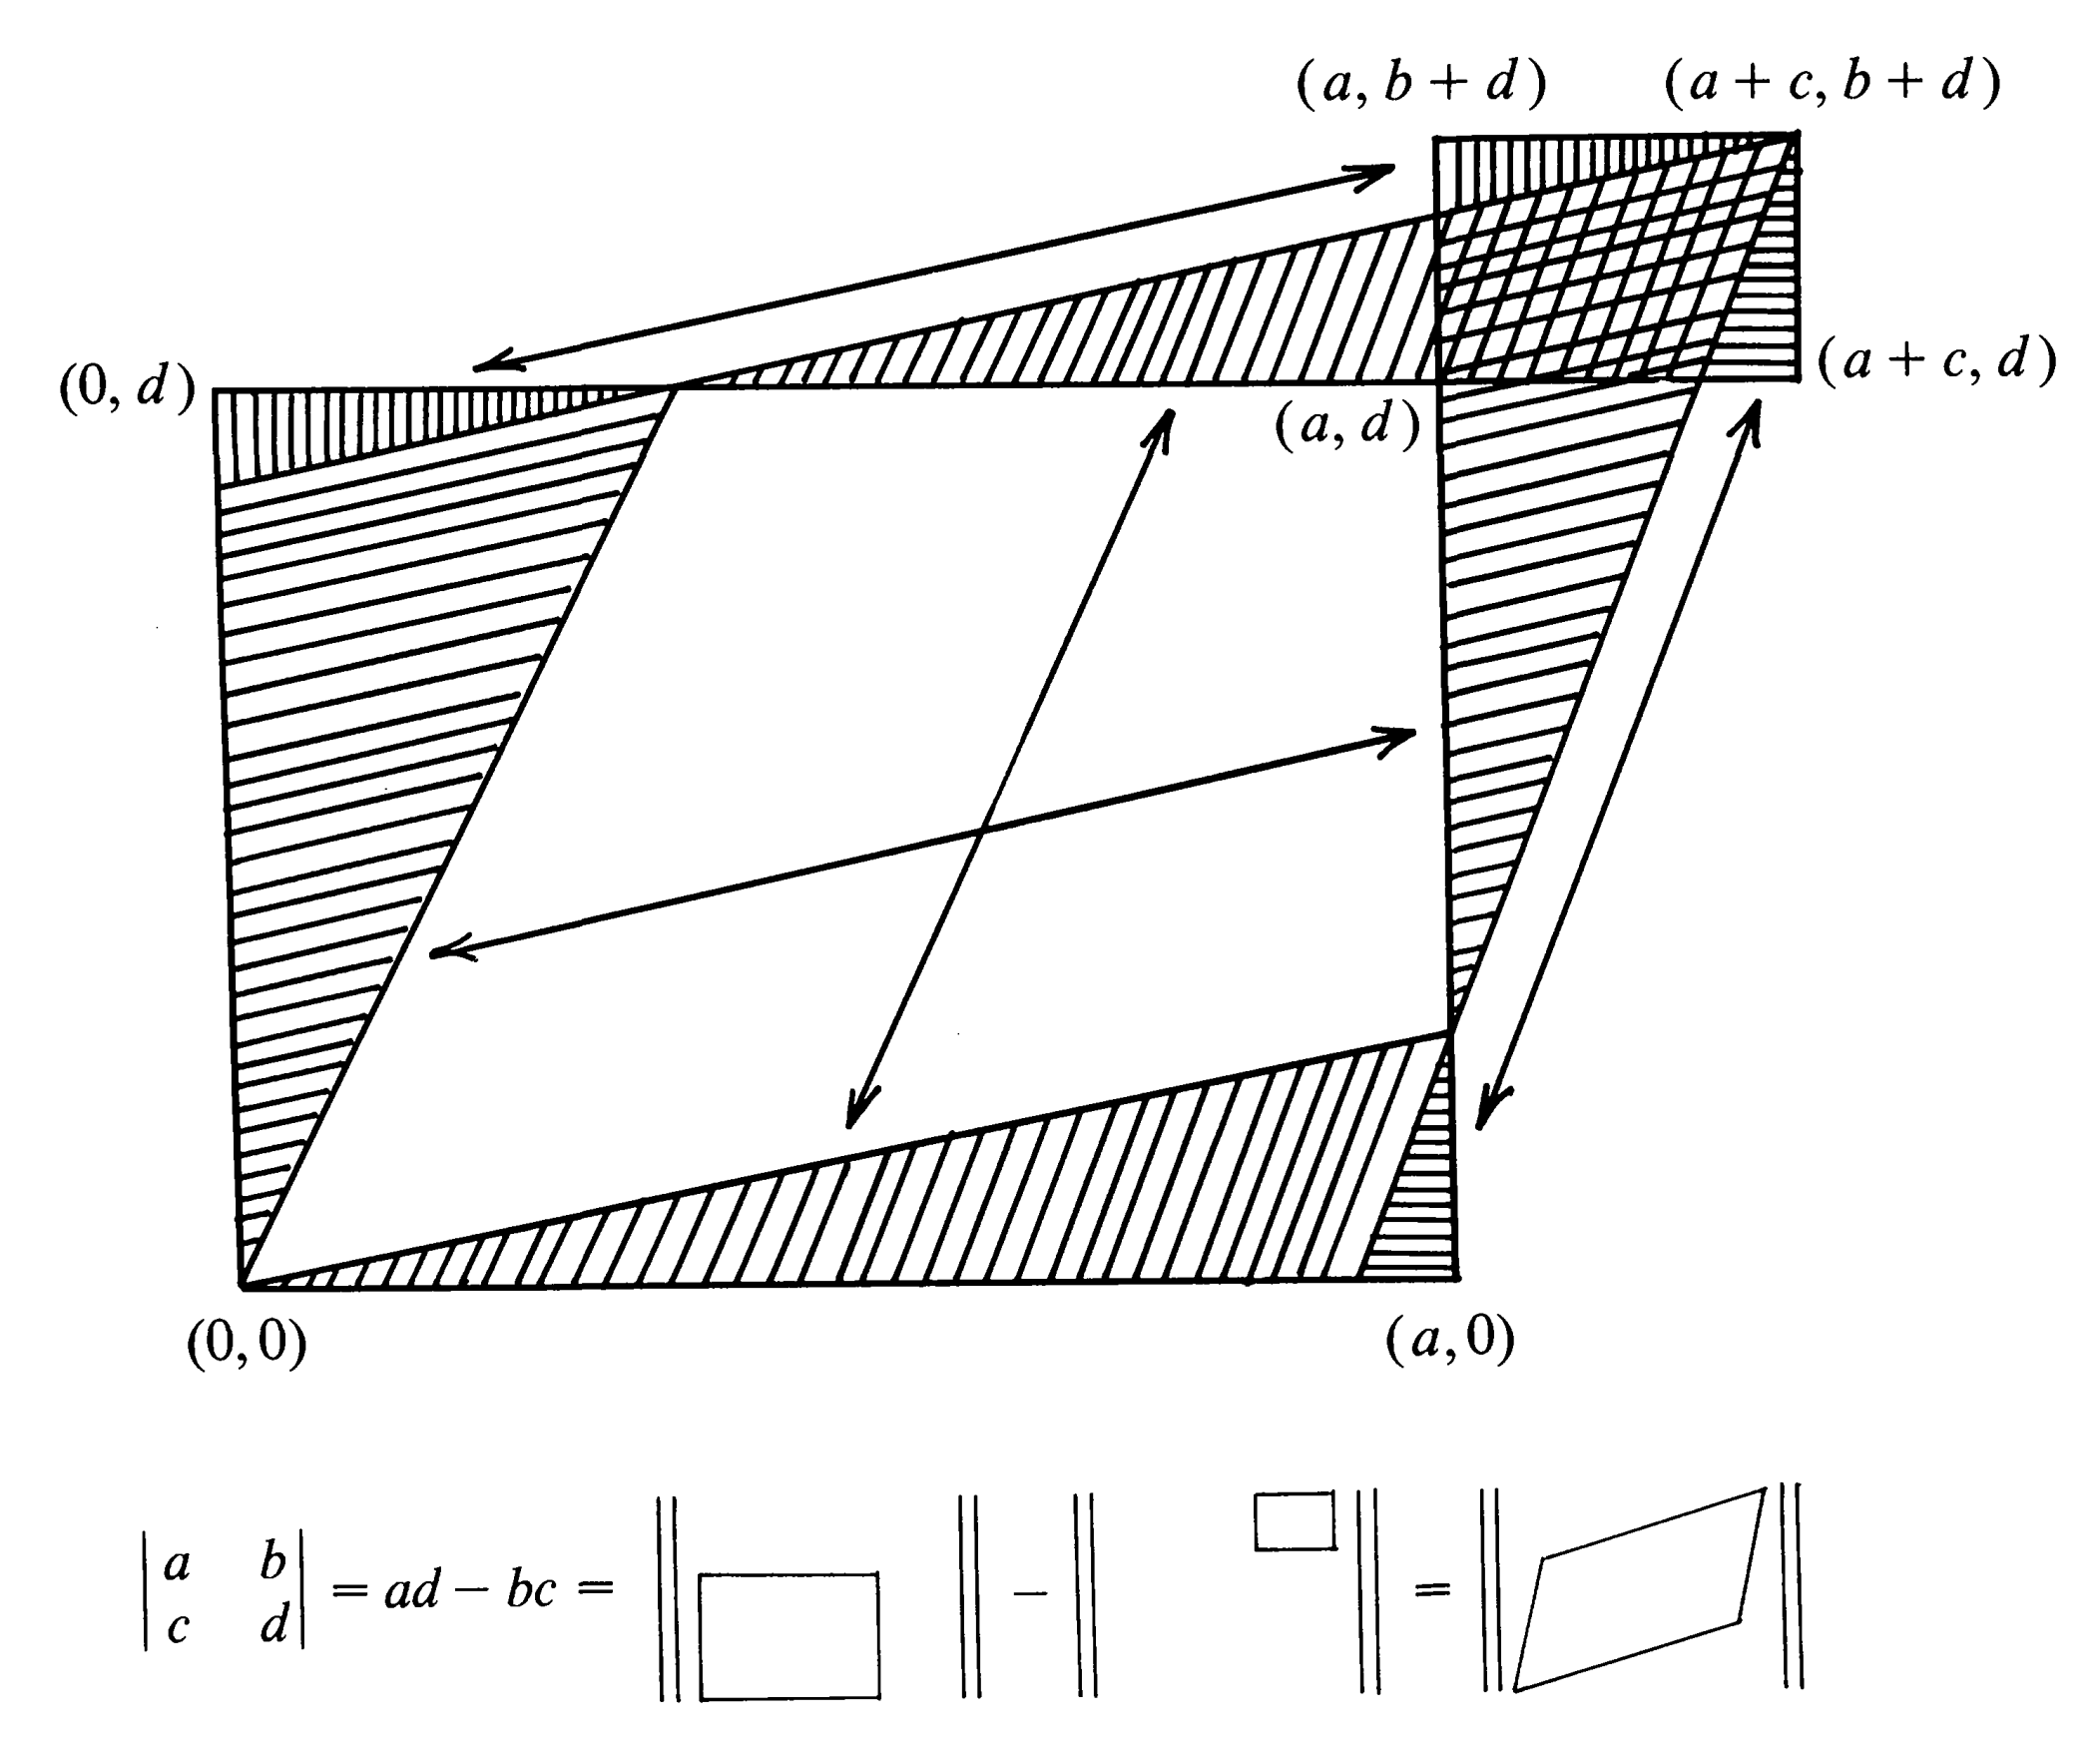
\includegraphics[width= 1\linewidth]{20}
		\caption{\small\textit{\color{toanhocdoisong}Hình $15$. Miền bao bởi đường cong kín.}}
		\vspace*{-10pt}
	\end{figure}
	Ứng với mỗi giá trị $t_i$, ta có một điểm $C(t_i)$ tương ứng trên đường cong.
	\vskip 0.1cm 
	Diện tích của đa giác tạo bởi các điểm $C(t_i)$ này có thể được tính theo công thức dây giày:
	\begin{align*}
		\frac{1}{2}\sum\limits_{i = 1}^n {x\left( {{t_{i - 1}}} \right)}
	\end{align*}
		Chú ý rằng khi đường cong kín thì $C(t_0)$ và $C(t_n)$ trùng nhau.
		\vskip 0.1cm
		Khi khoảng cách giữa các giá trị $t_i$ tiến tới $0$, ta có thể viết tổng này dưới dạng tích phân:
		\begin{align*}
			\frac{1}{2}\int_a^b {\left[ {x(t)y'(t) - y(t)x'(t)} \right]dt.}
		\end{align*}
		Những bạn đọc đã học qua giải tích vector sẽ biết đây là một công thức được suy ra từ định lý Green cho tích phân đường. Mặt khác, công thức dây giày cũng có thể được chứng minh bằng cách áp dụng công thức trên cho trường hợp đường cong kín là đường gấp khúc.
		\vskip 0.1cm
		Ví dụ, với trường hợp đường ellipse, ta có thể tính diện tích của miền bao bởi nó như sau:
		\begin{align*}
			A =& \frac{1}{2}\int_0^{2\pi } \left[ (a\cos t)(b\cos t) \right.\\
				&\left.- (b\sin t)( - a\sin t) \right]dt \\
				= &\frac{1}{2}ab\int_0^{2\pi } dt = \pi ab 
		\end{align*}
		\textbf{\color{toanhocdoisong}Bài tập}
		\vskip 0.1cm
		Sử dụng công thức tích phân trên để tính diện tích bao bởi các đường cong kín sau:
		$a)$ $(\sin2t,\sin t)$, $0\le t \le \pi$.
		\begin{figure}[H]
			\vspace*{-5pt}
			\centering
			\captionsetup{labelformat= empty, justification=centering}
			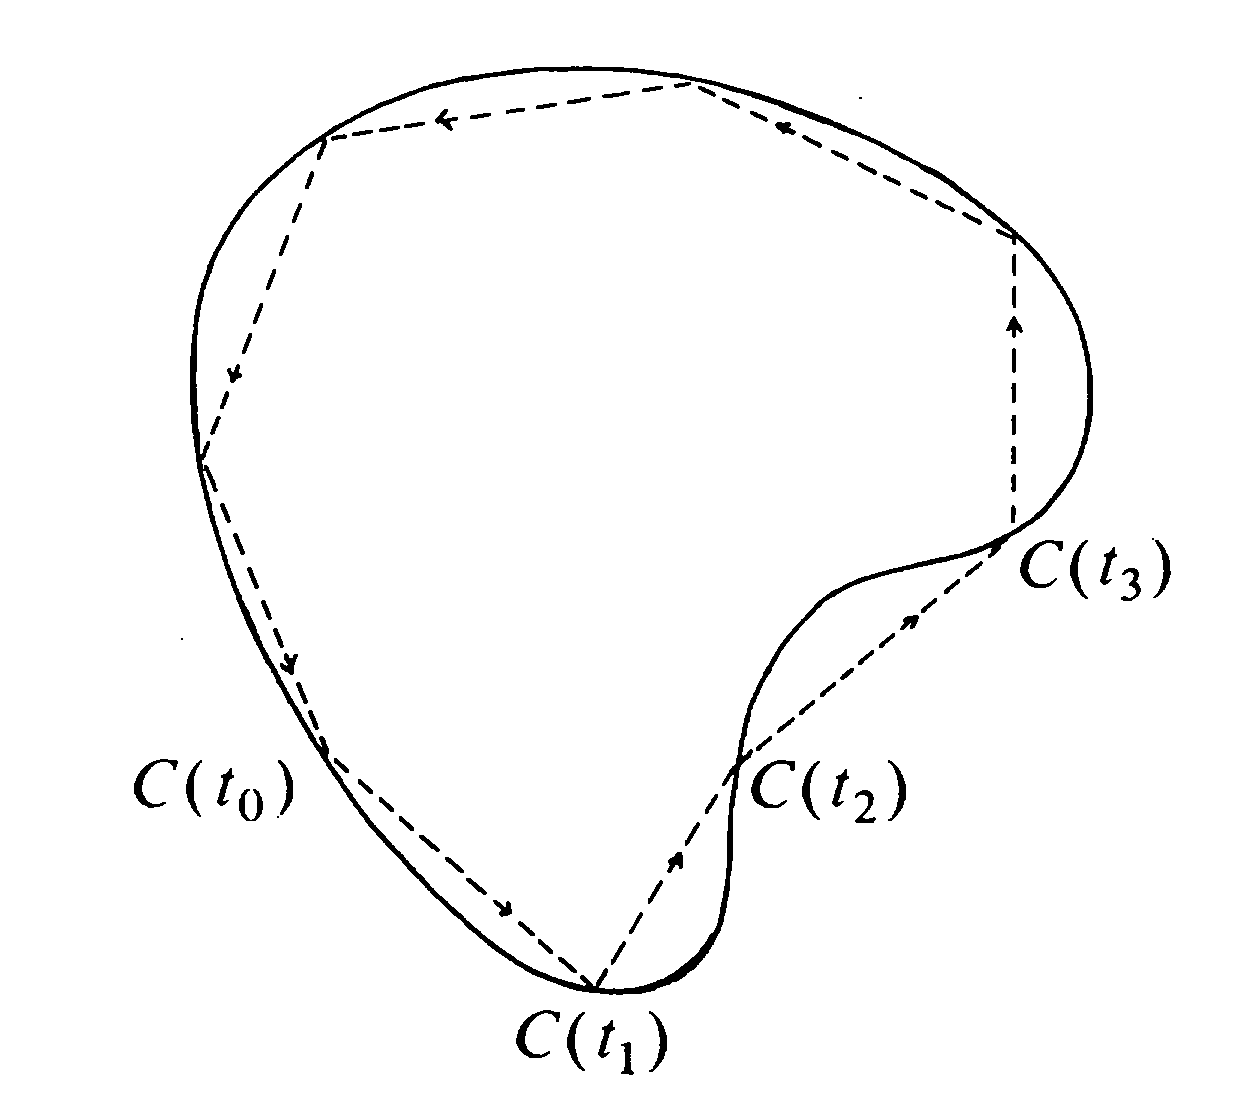
\includegraphics[width= 0.7\linewidth]{21}
			\vspace*{-10pt}
		\end{figure}
		$b)$ $(5\cos t-\cos5t,5\sin t- \sin5t),0 \le t \le 2\pi$.
		\begin{figure}[H]
			\vspace*{-5pt}
			\centering
			\captionsetup{labelformat= empty, justification=centering}
			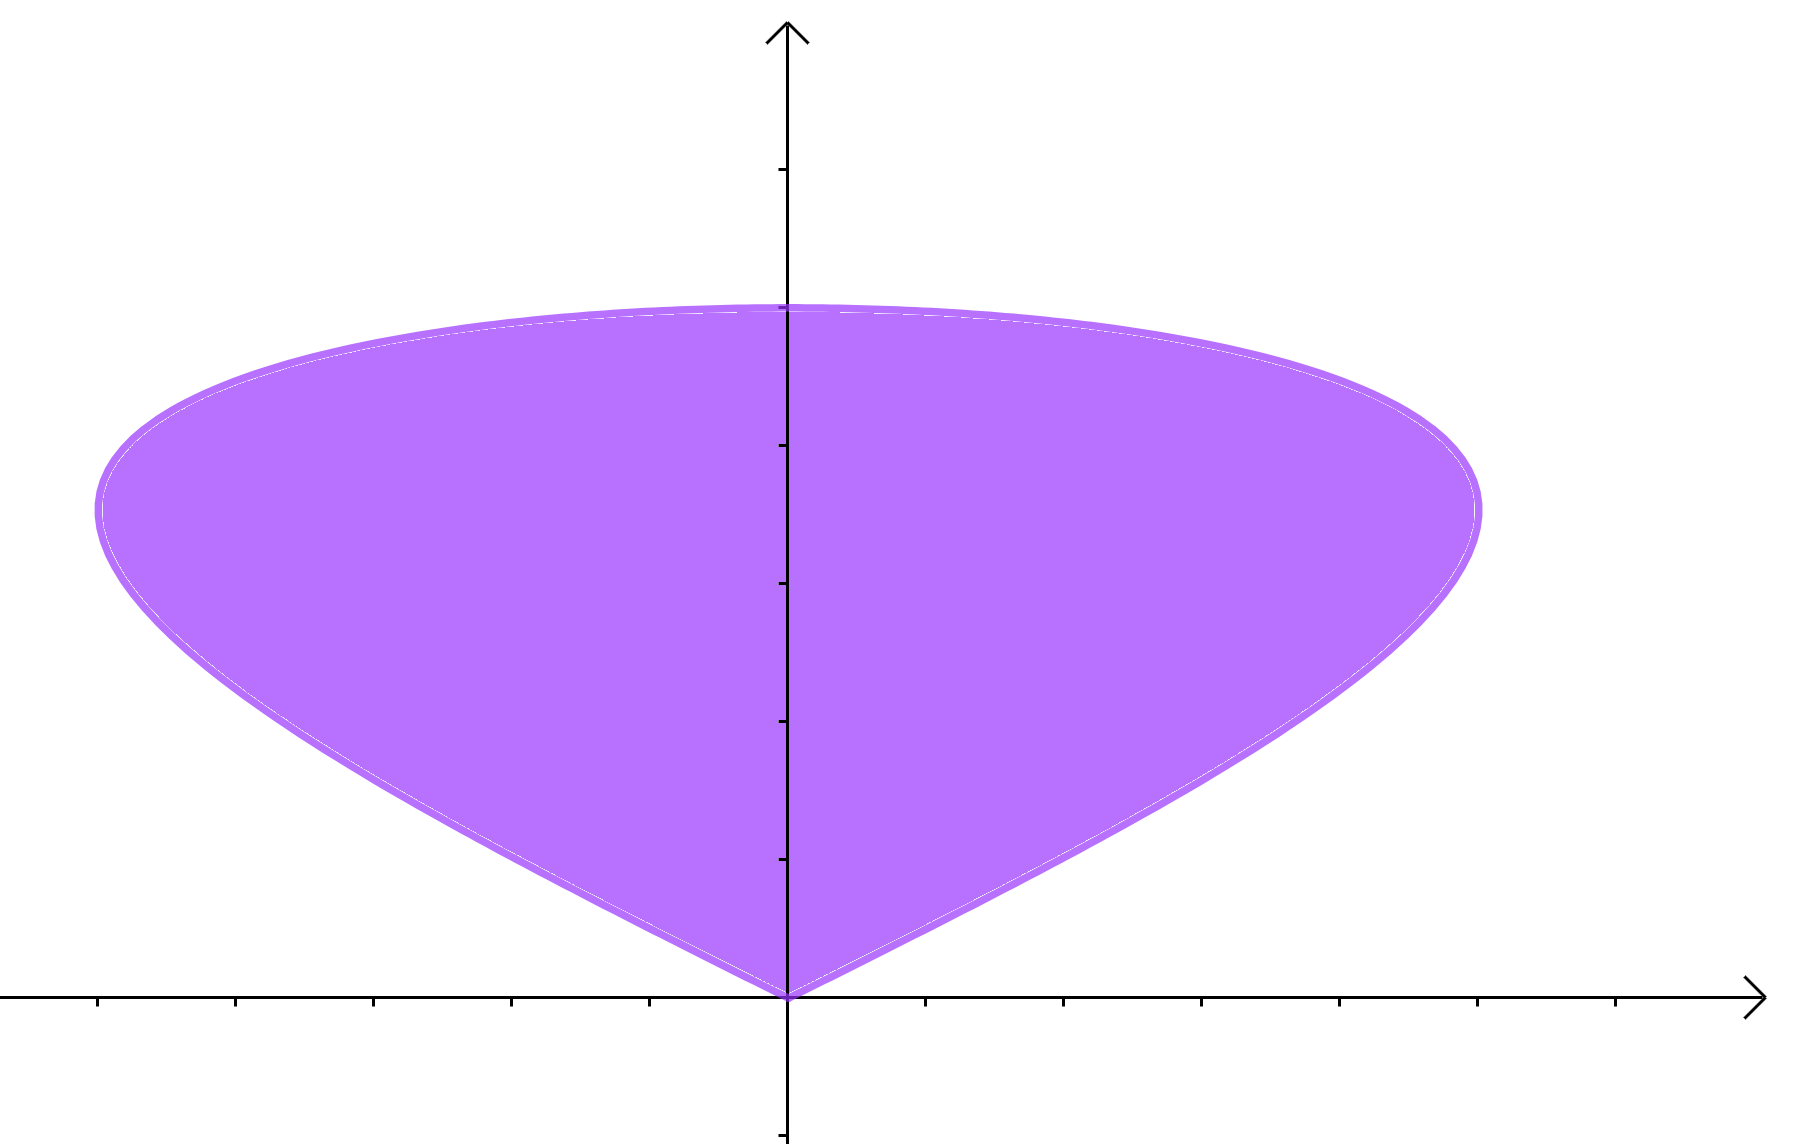
\includegraphics[width= 0.7\linewidth]{22}
			\vspace*{-10pt}
		\end{figure}
		$c)$ $(\cos^3 t,\sin^3t), 0\le t \le 2\pi$.
		\begin{figure}[H]
			\vspace*{-5pt}
			\centering
			\captionsetup{labelformat= empty, justification=centering}
			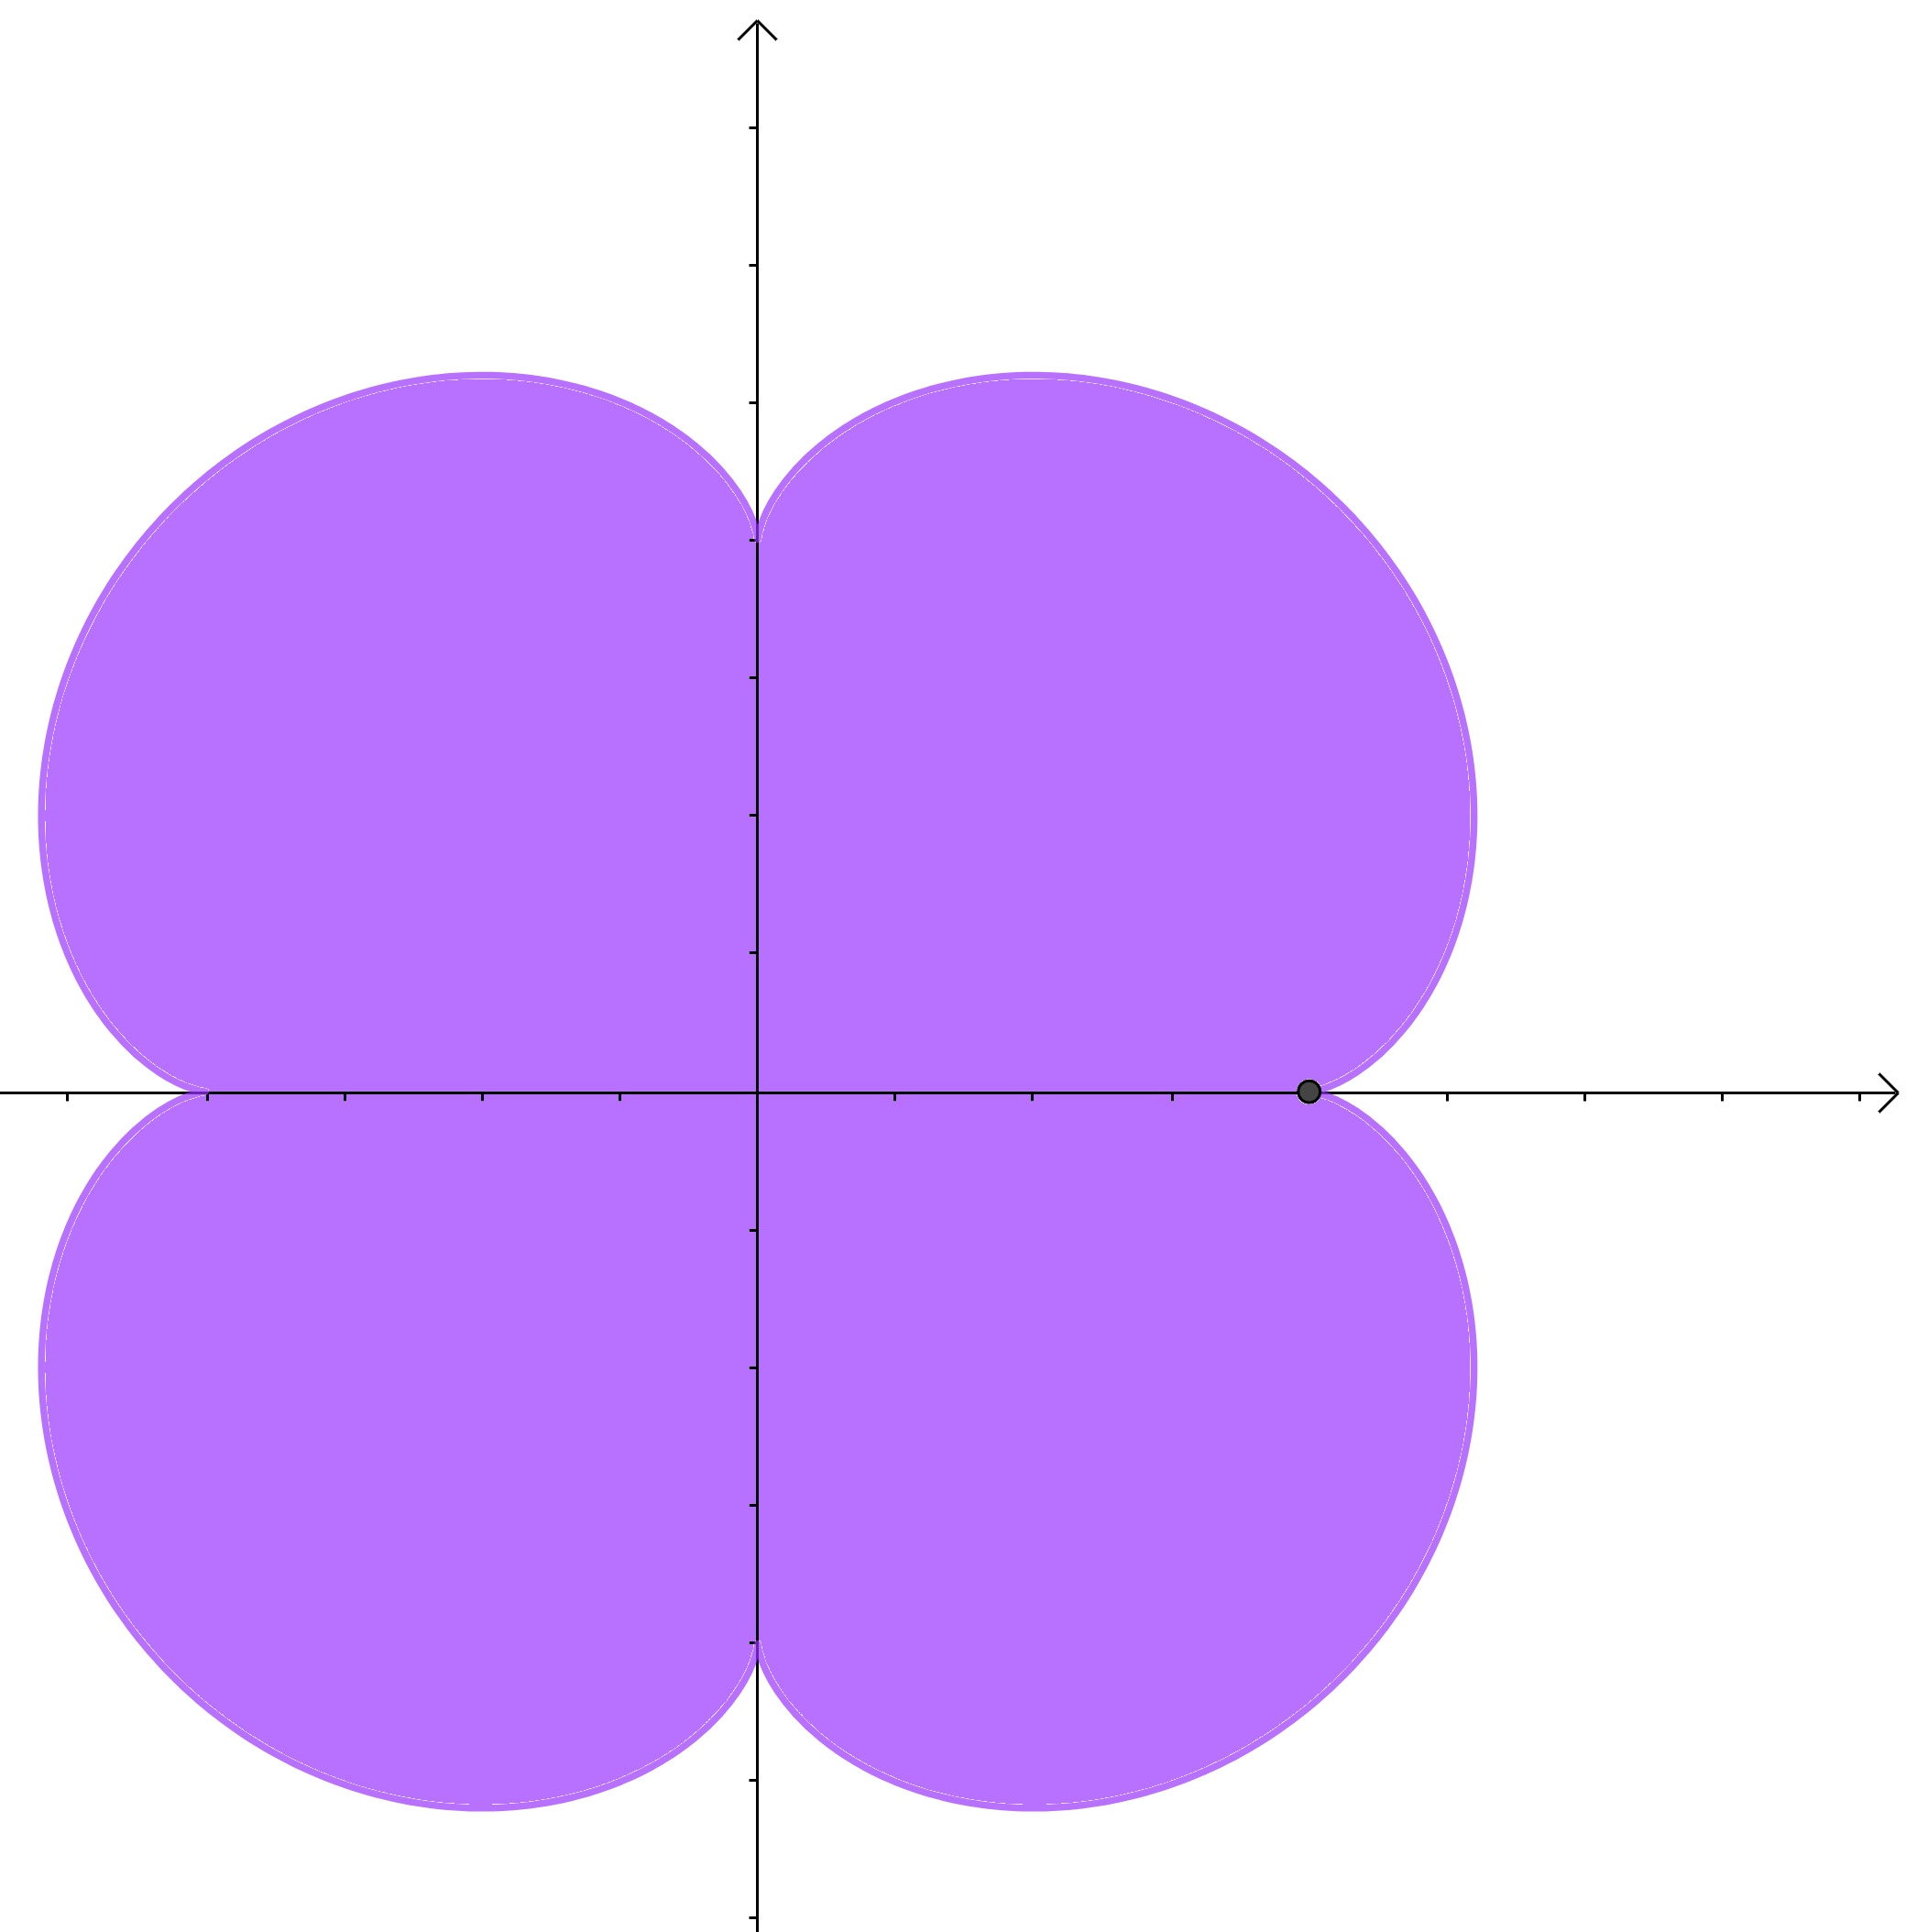
\includegraphics[width= 0.7\linewidth]{23}
			\vspace*{-10pt}
		\end{figure}
		$\pmb{4.}$ \textbf{\color{toanhocdoisong}Lời kết}
		\vskip 0.1cm
		Bài toán tích diện tích đa giác cũng như diện tích miền bao bởi đường cong kín là một đề tài tương đối thú vị khi giảng dạy về ứng dụng toán học cho học sinh phổ thông. Nó cũng có thể được kết hợp với hoạt động tiến hành đo đạc trắc địa thực tế trong các tiết học tích hợp hoặc cho học sinh tự thực hành ở nhà. Đồng thời, nội dung này cũng giúp học sinh làm quen với một số kiến thức sẽ được học ở môn giải tích bậc đại học.
		\vskip 0.1cm
		\textbf{\color{toanhocdoisong}Tài liệu tham khảo}
		\vskip 0.1cm
		[$1$] Braden, B. ($1986$). The Surveyor's Area Formula. \textit{College Mathematics Journal}, $17(4)$, $326–337$. \url{https://doi.org/10.1080/07468342.1986.11972974}
		\vskip 0.1cm
		[$2$] Lee, Y., \& Lim, W. ($2017$). Shoelace Formula: Connecting the Area of a Polygon and the Vector Cross Product. \textit{The Mathematics Teacher}, $110(8), 631-636$. \url{https://doi.org/10.5951/mathteacher.110.8.0631}
		\vskip 0.1cm
		[$3$] Leise, T. $(2007)$. As the Planimeter's Wheel Turns: Planimeter Proofs for Calculus Class. \textit{The College Mathematics Journal}, $38(1)$, $24-31$. \url{https://doi.org/10.1080/07468342.2007.11922214}
		\vskip 0.1cm
		[$4$] Stewart, J. ($2019$). \textit{Calculus : concepts and contexts}. Boston, Ma, Usa: Cengage.
\end{multicols}